\documentclass[12pt]{article}

% Paquetes esenciales
\usepackage[utf8]{inputenc}
\usepackage[T1]{fontenc}
\usepackage[english]{babel}
\usepackage{amsmath, amssymb, amsfonts, amsthm}
\newtheorem{proposition}{Proposition}
\newtheorem{definition}{Definition}
\usepackage{graphicx}
\usepackage{hyperref}
\usepackage{xcolor}
\usepackage{geometry}
\usepackage{fancyhdr}
\usepackage{setspace}
\usepackage[most]{tcolorbox}
\usepackage{listings}
\usepackage{tcolorbox}
\tcbuselibrary{breakable, skins}
\usepackage{minted} % Asegúrate de compilar con -shell-escape
\usepackage{etoolbox} 
\usepackage{xparse} % permite definir comandos con 
\usepackage[round,authoryear]{natbib}
\usepackage[ruled,vlined,linesnumbered]{algorithm2e}
\usepackage{booktabs}

% Code blocks
\definecolor{codegray}{gray}{0.95}
\lstset{
  backgroundcolor=\color{codegray},
  basicstyle=\ttfamily\small,
  frame=single,
  numbers=left,
  numberstyle=\tiny,
  tabsize=2,
  breaklines=true,
  showstringspaces=false
}

% Hipervínculos
\hypersetup{
    colorlinks=true,
    linkcolor=blue,
    urlcolor=blue,
    citecolor=blue
}

% \newtcolorbox{answerbox}{
%   colback=white,
%   colframe=black,
%   boxrule=0.8pt,
%   arc=3pt,
%   left=5pt,
%   right=5pt,
%   top=5pt,
%   bottom=5pt
% }

% \newcommand{\answer}[1]{\begin{answerbox}#1\end{answerbox}}

% Márgenes
\geometry{
  left=2.0cm,
  right=2.0cm,
  top=2.5cm,
  bottom=3.5cm
}

% Interlineado
\onehalfspacing

% Encabezado y pie de página
\usepackage{fancyhdr}
\pagestyle{fancy}
\fancyhf{}

% Encabezado y pie de página
\pagestyle{fancy}
\fancyhf{}
\newcommand{\headerinfo}{Doctorado en Economía\\2025}

\lhead{
  \begin{minipage}[c]{0.5\textwidth}
    \begin{tabular}{@{}l l@{}}
      \raisebox{0.01cm}{
\includegraphics[height=1.6cm]{figures/escudo_uch.jpeg}} &
      \begin{minipage}[c]{0.75\textwidth}
        \vspace{-1.5em} % Subir texto sin mover nada más
        \small
        Universidad de Chile\\Facultad de Economía y Negocios  
      \end{minipage}
    \end{tabular}
  \end{minipage}
}
\rhead{
  \small
  \headerinfo   
  \vspace{-1.7em} % Subir texto sin mover nada más
}

\rfoot{  
  \small
  \thepage}
\lfoot{}

% Ajustes de espacio
\setlength{\headheight}{51pt}  % espacio reservado para el encabezado
\setlength{\headsep}{25pt}     % espacio entre encabezado y texto

% Metadatos básicos (se redefinen desde main.tex)
\newcommand{\papertitle}{}
\newcommand{\paperauthors}{}
\newcommand{\paperroles}{}

% Comando para construir el encabezado
\newcommand{\maketitlepaper}{
  \begin{center}
    \Large \textbf{\papertitle} \\
    \vspace{1.em}
    \normalsize
    \paperauthors \\
    \vspace{0.8em}
    \hspace*{0.8em} % pequeña indentación izquierda
    \begin{minipage}{1.\textwidth} % ancho controlado para el bloque
      \raggedright
      \footnotesize
      \paperroles
    \end{minipage}
  \end{center}

  \vspace{-1.5em}
  \begin{flushright}
    \small \today
  \end{flushright}
  
  \vspace{0.02em}
  \hrule
  \vspace{2.5em}
}



%% ANSWER BLOCK
\tcbuselibrary{listings, minted}
\newtcolorbox{answerbox}[1][\textwidth]{
  enhanced,
  breakable,
  colback=white,
  colframe=black,
  boxrule=0.5pt,
  arc=3pt,
  left=8pt,
  right=8pt,
  top=8pt,
  bottom=8pt,
  boxsep=5pt,
  sharp corners,
  before skip=1em,
  after skip=1em,
  fonttitle=\bfseries,
  width=#1
}

% Asignatura correspondiente
\renewcommand{\headerinfo}{ENECO894\\Spring 2025}
\renewcommand{\papertitle}{Problem Set 1: Public Finances}
\renewcommand{\paperauthors}{
  Cristobal Donoso-Oliva\textsuperscript{1},
  Pablo Gutierrez\textsuperscript{2},
  Javiera Parada R.\textsuperscript{3},
  Juan Duarte A.\textsuperscript{3},
  Marcelo Montes M.\textsuperscript{3}
}
\renewcommand{\paperroles}{
  1. PhD Student in Economics \\
  2. Professor \\
  3. Teaching Assistants
}


\begin{document}
\maketitlepaper


\begin{abstract}
  \noindent This document presents the complete solution to Problem Set 1 of Public Finance, where each section corresponds to one problem of the assignment. Section~\ref{sec:intergenerational-mobility} investigates intergenerational income mobility in Chile by replicating the Two-Sample Two-Stage Least Squares (TSTSLS) framework of \citet{nunez2010mobility} with Murphy--Topel variance corrections across historical CASEN surveys (1987, 1990, and 2006), and extends the analysis to labor informality through rank--rank regressions and multiple imputation under residual-correlation scenarios. Section~\ref{sec:wealth-inequality} analyzes household wealth inequality using the 2021 Household Financial Survey (\textit{Encuesta Financiera de Hogares}, EFH) from the Central Bank of Chile; addressing fat Pareto tails, negative net worth, and extreme unit non-response, we implement the pseudo-maximum likelihood tail-adjustment methodology of \citet{vermeulen2018} combining survey microdata with the \textit{Forbes World's Billionaires} list and benchmarking wealth aggregates to National Accounts totals. Section~\ref{sec:bfm-methodology} moves beyond parametric Pareto assumptions by examining the non-parametric calibration framework of \citet{blanchet2022weight} (BFM), endogenously identifying the survey-tax merging point ($y^*$) via fractal grid binning, generalized Pareto interpolation, and antitonic regression to reconcile CASEN income microdata (2017 and 2022) with administrative tax tabulations from the Chilean Internal Revenue Service (\textit{Servicio de Impuestos Internos}, SII). Section~\ref{sec:conclusions} concludes by synthesizing the core findings and outlining broader methodological and policy implications for inequality measurement.
  
  \noindent All replication code, data processing pipelines, and estimation routines are open-source and publicly available at \url{https://github.com/crisdonoli/measuring-inequality}.
\end{abstract}
\newpage
\section{Intergenerational Income Mobility}\label{sec:intergenerational-mobility}
%! TEX root = ../main.tex
In this section, we study intergenerational income mobility in Chile with informality. In particular, we replicate the estimates of \citet{nunez2010mobility}: first-stage earnings equations (Table~A) and two-sample two-stage least squares (TSTSLS) elasticities (Table~1) using CASEN 1987, 1990 and 2006.

To account for the absence of linked father-son income records, we follow the TSTSLS methodology: historic earnings equations predict paternal income from retrospective characteristics reported by sons, and the predicted income enters a second-stage regression with a Murphy-Topel correction \citep{murphy1985estimation}.

Finally, we extend the analysis beyond the original paper in two directions: (i) rank-rank regressions by pension-contribution status, and (ii) multiple imputation of paternal income and affiliation under alternative residual-correlation scenarios \citep{vanbuuren2018flexible,kim2016statistical}.

\subsection{Historic Earnings Equations}\label{sec:first-stage}
For each historic year $t \in \{1987, 1990\}$ we estimate by OLS the log of monthly labor income. $E$ contains four indicators of completed schooling level: primary, secondary, technical and university; the omitted category is no schooling or incomplete primary. Age is denoted by $a$:
\begin{equation}
    L_{jt} = \alpha_t + E_{jt}^{\prime}\gamma_t + \delta_{1t}a_{jt} + \delta_{2t}a_{jt}^2 + u_{jt}, \quad L = \log y.
    \label{eq:earn-a}
\end{equation}
The extended specification adds occupation indicators $O$ for employer, self-employed and domestic service; employees and laborers are the occupational reference:
\begin{equation}
    L_{jt} = \alpha_t + E_{jt}^{\prime}\gamma_t + O_{jt}^{\prime}\pi_t + \delta_{1t}a_{jt} + \delta_{2t}a_{jt}^2 + u_{jt}.
    \label{eq:earn-b}
\end{equation}
The first-stage samples are males aged 15--55, employed ($o21=1$), with positive labor income: $N=18{,}769$ (1987) and $N=20{,}387$ (1990); with occupation the samples are $18{,}441$ and $20{,}354$ respectively.\footnote{See \texttt{source/mobility.py} (\texttt{recode\_1987}, \texttt{recode\_1990}, \texttt{build\_sample}) and \texttt{notebooks/07\_nunez\_miranda.ipynb}, Sec.~1. In 1987 income sums \textit{ysefaj}, \textit{yganaj} and \textit{yespaj}; in 1990 and 2006 it is \textit{ytrabaj}.} Table~\ref{tab:mob-a} reports the replication of Table~A: schooling coefficients are positive and increasing, and the estimates match the reference implementation to four decimals.\footnote{Reference values from the author's replication files; standard errors are HC1.}

\begin{table}[H]
    \centering
    \caption{First-stage earnings equations (Table~A)}\label{tab:mob-a}
    \begin{tabular}{lcc}
        \toprule
        & CASEN 1987 & CASEN 1990 \\
        \midrule
        Complete primary & 0.2538 [0.0124] & 0.2132 [0.0117] \\
        Complete secondary & 0.7564 [0.0141] & 0.6315 [0.0136] \\
        Complete technical & 1.0638 [0.0725] & 0.9426 [0.0404] \\
        Complete university & 1.7927 [0.0271] & 1.4808 [0.0284] \\
        Age & 0.0777 [0.0037] & 0.0657 [0.0035] \\
        Age$^2$ & -0.0008 [0.0001] & -0.0006 [0.0000] \\
        Constant & 8.1609 [0.0612] & 9.1366 [0.0578] \\
        Observations & 18,769 & 20,387 \\
        Adj.\ R-squared & 0.35 & 0.29 \\
        \bottomrule
    \end{tabular}
    \vspace{0.2em}
    \flushleft\footnotesize{\textit{Note:} Dependent variable: log earnings. HC1 robust standard errors in brackets.}
\end{table}

\subsection{TSTSLS Elasticities}\label{sec:tsts}
In CASEN 2006, retrospective questions record paternal schooling (\textit{t14a}) and occupation (\textit{t15a}), recoded into the first-stage indicators; the son's own schooling is not used and co-residence is not required. Sons aged 25--35 are linked to 1990 coefficients and sons aged 36--40 to 1987 coefficients. Predicted paternal log income at age 40 is:
\begin{equation}
    \widehat{L}^{40}_{pi} = \widehat{\alpha}_t + E_{pi}^{\prime}\widehat{\gamma}_t + O_{pi}^{\prime}\widehat{\pi}_t + 40\widehat{\delta}_{1t} + 40^2\widehat{\delta}_{2t}.
    \label{eq:pred-father}
\end{equation}
To combine years, the prediction is centered on each historic sample's indicator means, so the constant and common age terms cancel:
\begin{equation}
    \widetilde{L}_{pi} = (E_{pi}-\bar{E}_t)^{\prime}\widehat{\gamma}_t + (O_{pi}-\bar{O}_t)^{\prime}\widehat{\pi}_t.
    \label{eq:centered}
\end{equation}
The second stage regresses demeaned son log income on predicted paternal income with an age profile:
\begin{equation}
    L_{hi}-\bar{L}_h = b_0 + \beta\widetilde{L}_{pi} + b_1a_{hi} + b_2a_{hi}^2 + \varepsilon_i.
    \label{eq:second}
\end{equation}
Table~\ref{tab:mob-1} replicates Table~1 over $N=11{,}178$ sons aged 25--40.\footnote{See \texttt{source/mobility.py} (\texttt{two\_step\_elasticity}) and \texttt{notebooks/07\_nunez\_miranda.ipynb}, Sec.~2. The Murphy-Topel term adds $DVD^{\prime}$ to the second-stage HC1 variance, where $D$ measures sensitivity to first-stage parameters and means; independence between surveys is assumed.} With education only, a 1\% higher predicted paternal income is associated with 0.83\% higher son income (0.61\% adding occupation).

\begin{table}[H]
    \centering
    \caption{TSTSLS income elasticities (Table~1)}\label{tab:mob-1}
    \begin{tabular}{lcccc}
        \toprule
        Son's age & Education & obs.\ & Education + occupation & obs.\ \\
        \midrule
        25--30 & 0.748 [0.042] & 3,017 & 0.471 [0.036] & 3,017 \\
        31--35 & 0.902 [0.041] & 3,550 & 0.670 [0.033] & 3,550 \\
        36--40 & 0.835 [0.038] & 4,611 & 0.669 [0.035] & 4,611 \\
        25--40 & 0.833 [0.024] & 11,178 & 0.614 [0.021] & 11,178 \\
        31--40 & 0.862 [0.028] & 8,161 & 0.669 [0.025] & 8,161 \\
        \bottomrule
    \end{tabular}
    \vspace{0.2em}
    \flushleft\footnotesize{\textit{Note:} HC1 standard errors with Murphy-Topel correction in brackets.}
\end{table}

\subsection{Rank-Rank Regressions and Informality}\label{sec:rank}
For each age group, percentiles are assigned among imputed fathers and among sons in that group, with average ranks for ties:
\begin{equation}
    R_{pi} = 100\,\frac{\mathrm{rank}(\widetilde{L}_{pi})}{N_g}, \qquad R_{hi} = 100\,\frac{\mathrm{rank}(y_{hi})}{N_g}.
    \label{eq:ranks}
\end{equation}
The rank-rank slope comes from $R_{hi} = \alpha + \beta_R R_{pi} + e_i$ (with an age-controls variant as check).\footnote{See \texttt{source/mobility.py} (\texttt{rank\_rank}) and \texttt{notebooks/07\_nunez\_miranda.ipynb}, Sec.~3.} Table~\ref{tab:mob-rank} reports the 25--40 group ($N=11{,}178$): the total slope is 0.325 with education (Spearman 0.319). Sons are classified as formal if contributing ($o29 \in 1$--$5$, $N=8{,}241$) and informal if affiliated without contributing or unaffiliated ($o29 \in 6$--$7$, $N=2{,}823$); both sectors use ranks from the full age group.

\begin{table}[H]
    \centering
    \caption{Rank-rank slopes, sons aged 25--40}\label{tab:mob-rank}
    \begin{tabular}{lccccc}
        \toprule
        Predictors & Total & Formal & Informal & Spearman (inf.) & $N$ inf.\ \\
        \midrule
        Education & 0.325 [0.009] & 0.320 [0.010] & 0.295 [0.021] & 0.250 & 2,823 \\
        Education + occupation & 0.322 [0.009] & 0.313 [0.010] & 0.329 [0.020] & 0.280 & 2,823 \\
        \bottomrule
    \end{tabular}
    \vspace{0.2em}
    \flushleft\footnotesize{\textit{Note:} Conditional HC1 standard errors in brackets. Spearman column refers to the informal sector.}
\end{table}

Figure~\ref{fig:rank-sector} plots the fitted lines: with education, ten more paternal percentile points are associated with 3.25 points for the child in the total and 2.95 among informal sons; adding occupation the figures are 3.22 and 3.29. The direction of the gap reverses and conditional contrasts do not reject equality at 5\%, so no general claim of higher mobility among informal sons follows.

\begin{figure}[H]
    \centering
    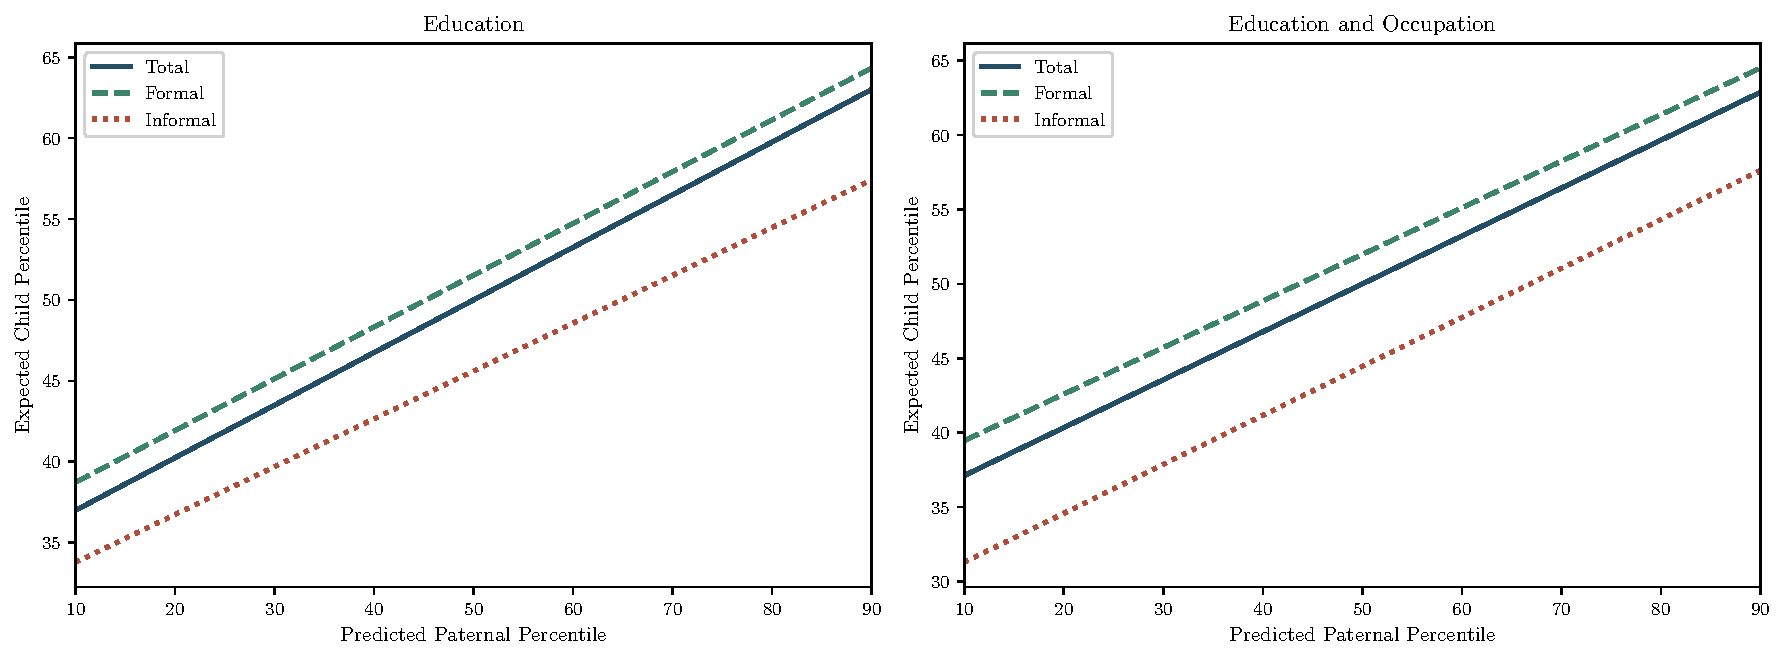
\includegraphics[width=0.95\textwidth]{../../figures/p1/rank_sector.pdf}
    \caption{Rank-rank fitted lines by sector (sons 25--40). Predicted paternal percentile vs.\ expected son percentile.}\label{fig:rank-sector}
\end{figure}

\subsection{Multiple Imputation of Paternal Income and Status}\label{sec:mi}
We restrict this extension to 6,498 sons aged 25--35 with known pension status. Paternal formality is proxied by historic affiliation ($o11 \in 1$--$6$ vs.\ $7$) while the son's is current contribution ($o29$); the two indicators differ in meaning. Log incomes follow a bivariate normal residual model with assumed correlation $\rho$:
\begin{equation}
    L_{pi} = \mu_{pi} + \varepsilon_{pi}, \quad L_{hi} = \mu_{hi} + \varepsilon_{hi}, \quad (\varepsilon_p,\varepsilon_h)^{\prime} \sim N_2(0,\Sigma_\rho).
    \label{eq:mi-model}
\end{equation}
Status follows a logistic model in predictors, age profile and log income. For each scenario $\rho \in \{0, 0.3, 0.6\}$ we generate $M=100$ versions: coefficients and variances are drawn from normal and inverse-chi-square posteriors, then paternal income and affiliation are imputed conditional on the son's observed residual.\footnote{See \texttt{source/mobility.py} (\texttt{multiple\_imputation}, seed 17102026) and \texttt{notebooks/07\_nunez\_miranda.ipynb}, Sec.~4. Same data-generating process as the reference implementation; the random engine differs so figures match within Monte Carlo error, not exactly.}

Within each imputation, paternal percentiles are recomputed over all 6,498 cases and rank-rank slopes are estimated for the four father-son combinations (F-F, F-I, I-F, I-I), then pooled with Rubin's rules.\footnote{Combined slope $\bar{\beta} = M^{-1}\sum \hat{\beta}^{(m)}$, total variance $T = \bar{U} + (1+M^{-1})B$ with Barnard-Rubin degrees of freedom.} Table~\ref{tab:mob-mi} shows the cotizante-son criterion: the affiliated-father/contributing-son slope is 0.168, 0.355 and 0.564 under $\rho = 0$, $0.3$ and $0.6$. The spread across scenarios reflects non-identified residual dependence, not something more imputations would resolve.

\begin{table}[H]
    \centering
    \caption{Multiple imputation: combined slopes by scenario (son = contributor)}\label{tab:mob-mi}
    \begin{tabular}{lcccc}
        \toprule
        $\rho$ & Father--son & Slope & 95\% interval & Mean $N$ \\
        \midrule
        0.0 & F-F & 0.168 & [0.130; 0.206] & 3,677 \\
        0.0 & F-I & 0.220 & [0.128; 0.311] & 971 \\
        0.0 & I-F & 0.116 & [0.045; 0.186] & 1,268 \\
        0.0 & I-I & 0.131 & [0.007; 0.256] & 582 \\
        0.3 & F-F & 0.355 & [0.319; 0.390] & 3,683 \\
        0.3 & F-I & 0.492 & [0.411; 0.572] & 966 \\
        0.3 & I-F & 0.294 & [0.229; 0.360] & 1,262 \\
        0.3 & I-I & 0.431 & [0.323; 0.538] & 587 \\
        0.6 & F-F & 0.564 & [0.535; 0.593] & 3,688 \\
        0.6 & F-I & 0.726 & [0.667; 0.785] & 960 \\
        0.6 & I-F & 0.490 & [0.430; 0.549] & 1,257 \\
        0.6 & I-I & 0.675 & [0.598; 0.753] & 593 \\
        \bottomrule
    \end{tabular}
    \vspace{0.2em}
    \flushleft\footnotesize{\textit{Note:} 100 imputations per scenario; F = affiliated father / contributing son. Intervals use Barnard-Rubin degrees of freedom.}
\end{table}

Figure~\ref{fig:mi-sens} shows the sensitivity: slopes rise with $\rho$ in all four groups, and the ordering F-F $<$ F-I is descriptive, not a tested difference. Conditioning on income-related states selects different distributions, so a higher slope means stronger relative association within the group, not a better outcome or upward mobility.

\begin{figure}[H]
    \centering
    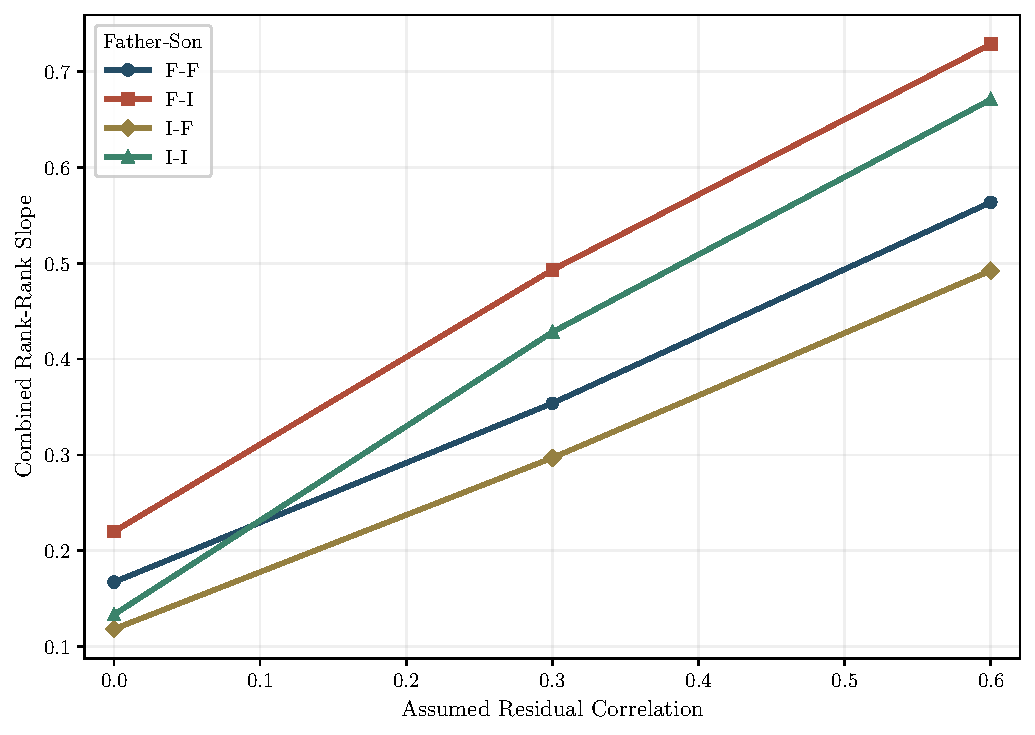
\includegraphics[width=0.70\textwidth]{../../figures/p1/sensibilidad_MI.pdf}
    \caption{Sensitivity of combined slopes to the assumed residual correlation. F = affiliated father / contributing son.}\label{fig:mi-sens}
\end{figure}


\newpage
\section{Wealth Inequality}\label{sec:wealth-inequality}
%! TEX root = ../main.tex
In this section, we measure wealth inequality in Chile. In particular, we analyze the 2021 cross-section using data from the Household Financial Survey (\textit{Encuesta Financiera de Hogares}, EFH) published by the Central Bank of Chile \citep{bcentral2021efh}.

To account for differential unit non-response and extreme under-reporting at the upper tail of the wealth distribution, a pervasive limitation of survey data, we implement the tail-correction methodology developed by \citet{vermeulen2018}. Specifically, this approach fits a Pareto distribution to the tail by combining survey observations with external data on ultra-high-net-worth individuals from the \textit{Forbes World's Billionaires} list \citep{forbes2021billionaires,forbes2021kaggle}.

Finally, we compare the baseline survey estimates with the Pareto-corrected wealth shares and discuss the sensitivity of the results.

\subsection{Measuring wealth inequality}\label{sec:measuring-wealth}
Following standard international guidelines \citep[e.g.,][]{oecd2013wealth} and the methodology of the Central Bank of Chile for the EFH, net wealth (or net worth) of household $i$, denoted by $W_i$, is defined as the total value of all its non-financial and financial assets minus total outstanding liabilities:
\begin{equation}
    W_i = A_i - L_i = (A_i^{\text{NF}} + A_i^{\text{F}}) - (L_i^{\text{M}} + L_i^{\text{NM}}),
    \label{eq:net_wealth}
\end{equation}
where:
\begin{itemize}
    \item $A_i^{\text{NF}}$ denotes \textit{non-financial assets}, primarily comprising main residence, secondary real estate properties, and other tangible assets (vehicles, machinery, and self-employment business assets).
    \item $A_i^{\text{F}}$ denotes \textit{financial assets}, including checking and savings accounts, mutual and pension funds (voluntary retirement savings), stocks, bonds, and business equity holdings.
    \item $L_i^{\text{M}}$ represents \textit{mortgage debt} secured against real estate (housing and other properties).
    \item $L_i^{\text{NM}}$ represents \textit{non-mortgage liabilities}, covering consumer loans, credit cards, education debt, and informal or retail commercial credit.
\end{itemize}
Under this definition, gross wealth is $A_i = A_i^{\text{NF}} + A_i^{\text{F}}$, and net wealth $W_i$ can be negative for over-indebted households ($L_i > A_i$). 

Three main empirical and methodological challenges arise when measuring wealth inequality under this framework. First, wealth is substantially more concentrated than income because it accumulates over the life cycle and across generations. Consequently, the wealth distribution exhibits a fat Pareto tail, meaning that undersampling or non-response among the wealthiest households exerts a first-order downward bias on inequality estimates. Second, measuring wealth components through surveys is subject to severe measurement error and item non-response, requiring complex imputation procedures that inevitably introduce estimation uncertainty. Third, because net wealth can take negative values, standard summary indices such as the Gini coefficient \citep{gini1912variabilita} lose some of their desirable axiomatic properties (e.g., boundedness between 0 and 1; see Appendix \ref{app:gini-negative} for a mathematical proof). To face this, the empirical literature primarily relies on percentile wealth shares (such as the share of wealth held by the top 1\% or 10\%), 
\begin{equation}
    S_P = \frac{\sum_{i=1}^N w_i W_i \cdot \mathbf{1}\{W_i \in P\}}{\sum_{i=1}^N w_i W_i},
    \label{eq:wealth_share}
\end{equation}
where $w_i$ denotes the survey sampling weight of household $i$, $\mathbf{1}\{\cdot\}$ is the indicator function, and $P$ represents the subset of households belonging to a specific percentile bracket (e.g., the top 1\%, top 10\%, or bottom 50\%).

While wealth shares directly capture concentration at key points of the distribution, they do not provide a single scalar summary of dispersion across the entire population. In this context, reporting the wealth share of the bottom 50\% is essential to provide a balanced assessment of concentration and to evaluate disparity across the entire distribution. 

Because positive and negative net wealth values offset each other in the summation, the survey-based aggregate denominator ($\sum_{i=1}^N w_i W_i$) can become highly volatile or sensitive to extreme debts. Household surveys also systematically under-report aggregate financial and non-financial assets relative to macroeconomic totals. To address these limitations and follow standard distribution national accounts (DINA) practices, we anchor the denominator to the aggregate household net wealth reported in the National Accounts by the Central Bank of Chile \citep{bcentral2021financialaccounts}. The rescaled wealth share is thus defined as:
\begin{equation}
    S_P^{\text{NA}} = \frac{\sum_{i=1}^N w_i W_i \cdot \mathbf{1}\{W_i \in P\}}{W^{\text{NA}}},
    \label{eq:wealth_share_na}
\end{equation}
where $W^{\text{NA}}$ denotes the total household net wealth benchmark from the National Accounts. 

\subsection{Addressing the Differential Unit Non-Response Problem}\label{sec:vermeulen}
Sample surveys suffer from missing data at the upper tail because ultra-wealthy individuals exhibit disproportionately higher unit non-response rates and under-report sensitive assets (Section~\ref{sec:measuring-wealth}). To correct for this truncation and obtain an accurate representation of top wealth shares, \citet{vermeulen2018} proposed a semi-parametric tail-correction methodology that augments survey microdata with external rich lists (such as the \textit{Forbes World's Billionaires} rankings) and estimates an augmented Pareto distribution.

Because power-law behavior holds strictly at the upper tail, the Pareto model is fitted only for wealth levels exceeding a predetermined lower threshold, $w_{\min}$ (see Appendix \ref{app:pareto-foundations} for microeconomic foundations). In practice, $w_{\min}$ is chosen based on visual inspection of log-log rank plots (detecting where the linearity of the tail begins) or through goodness-of-fit heuristics \citep[e.g.,][]{clauset2009power,vermeulen2018}.

Formally, for any wealth level $w \ge w_{\min}$, the cumulative distribution function (CDF), denoted by $F(w)$, and the probability density function (PDF), denoted by $f(w)$, of a Type-I Pareto distribution are defined as:
\begin{align}
    F(w) &= 1 - \left(\frac{w_{\min}}{w}\right)^\alpha, \label{eq:pareto_cdf} \\
    f(w) &= \frac{\mathrm{d}F(w)}{\mathrm{d}w} = \frac{\alpha w_{\min}^\alpha}{w^{\alpha + 1}}, \label{eq:pareto_pdf}
\end{align}
where $w_{\min} > 0$ represents the tail cutoff point and $\alpha > 0$ is the Pareto shape parameter (tail index), governing the thickness of the tail (with smaller values of $\alpha$ indicating a heavier tail and higher wealth concentration). The complementary cumulative distribution function (or survival function), which gives the probability that an individual's wealth exceeds $w$, is therefore expressed as:
\begin{equation}
    P(W > w) = 1 - F(w) = \left(\frac{w_{\min}}{w}\right)^\alpha.
    \label{eq:pareto_survival}
\end{equation}

The estimation and imputation procedure is summarized in Algorithm \ref{alg:vermeulen}. To estimate the Pareto tail index $\alpha$, we apply the pseudo-maximum likelihood (PML) estimator developed by \citet{vermeulen2018}. Standard Maximum Likelihood cannot be applied directly because survey observations represent sampled clusters with expansion weights $w_i$, whereas the Forbes list represents an exhaustive, unweighted census ($w_j^F = 1$) of extreme wealth. The PML log-likelihood function combines both data sources by weighting each survey contribution by its sampling weight while treating billionaire records as self-representing:
\begin{equation}
    \ln \mathcal{L}(\alpha) = \sum_{k=1}^n w_k \ln f(W_k; \alpha) + \sum_{j=1}^M \ln f(W_j^F; \alpha).
    \label{eq:pml_loglik}
\end{equation}
Substituting the Pareto density $f(w; \alpha) = \alpha w_{\min}^\alpha w^{-(\alpha + 1)}$ and solving the first-order condition $\frac{\partial \ln \mathcal{L}}{\partial \alpha} = 0$ yields the closed-form estimator:
\begin{equation}
    \hat{\alpha} = \frac{\sum_{k=1}^n w_k + M}{\sum_{k=1}^n w_k \ln\left(\frac{W_k}{w_{\min}}\right) + \sum_{j=1}^M \ln\left(\frac{W_j^F}{w_{\min}}\right)}.
    \label{eq:alpha_pml}
\end{equation}
Econometrically, $\hat{\alpha}^{-1}$ corresponds to the weighted average relative distance of log wealth above the cutoff $w_{\min}$. When wealth in the tail is heavily concentrated far above $w_{\min}$, the denominator expands, resulting in a lower $\hat{\alpha}$ (i.e., a heavier Pareto tail, which implies a higher concentration of aggregate wealth and greater inequality).

As a complement to PML, we also use the bias-corrected rank-size regression of \citet{gabaix2011rank}\footnote{See \texttt{source/pareto.py:L5-L38} (\texttt{estimate\_alpha\_pareto}, \texttt{method="reg"}).}. Sorting the combined tail sample descending with cumulative weights $R_k$, the Pareto implies $\ln(R_k/N)\approx -\alpha\ln(W_k)+\alpha\ln w_{\min}$, so $\alpha$ is minus the OLS slope of log-rank on log-wealth. We use the $1/2$ shift, $\ln((R_k-0.5w_k)/N)$ on $\ln W_k$, to reduce small-sample bias at the very top.

\begin{algorithm}[H]
    \caption{Vermeulen (2018) Tail-Correction Procedure}\label{alg:vermeulen}
    \SetAlgoLined
    \KwIn{Survey microdata $\{(W_i, w_i)\}_{i=1}^N$; external Forbes list $\{W_j^F\}_{j=1}^M$; tail threshold $w_{\min}$; national accounts benchmark $W^{\text{NA}}$.}
    \KwOut{Pareto tail index $\hat{\alpha}$; pseudo-observations with weights; corrected top wealth shares $\hat{S}_P$.}
    
    \BlankLine
    \tcp{Step 1: Sample Selection above Tail Threshold}
    Extract survey households satisfying $W_i \ge w_{\min}$, indexing them by $k = 1, \dots, n$, with weights $w_k$\;
    Include external Forbes individuals with weight $w_j^F = 1$, since they represent the full enumeration of known billionaires ($W_j^F \ge w_{\min}$)\;
    
    \BlankLine
    \tcp{Step 2: Estimation of the Pareto Tail Index ($\alpha$)}
    Fit a Type-I Pareto distribution $P(W \ge w) = (w_{\min} / w)^\alpha$ on the combined sample by pseudo-maximum likelihood (or weighted OLS on the rank log-log regression):
    \[
        \hat{\alpha} = \frac{\sum_{k=1}^n w_k + M}{\sum_{k=1}^n w_k \ln(W_k / w_{\min}) + \sum_{j=1}^M \ln(W_j^F / w_{\min})}
    \]
    
    \BlankLine
    \tcp{Step 3: Replacing or Augmenting the Survey Tail}
    Replace the empirical survey observations above $w_{\min}$ with synthetic pseudo-observations generated from the estimated Pareto density $f(w; \hat{\alpha}) = \hat{\alpha} w_{\min}^{\hat{\alpha}} w^{-(\hat{\alpha}+1)}$, calibrating total population weights to match the aggregate tail mass $N_{\text{tail}} = \sum_{k=1}^n w_k$\;
    
    \BlankLine
    \tcp{Step 4: Recomputing Corrected Wealth Shares}
    Evaluate aggregate tail wealth $\hat{W}_{\text{tail}} = N_{\text{tail}} \cdot \frac{\hat{\alpha}}{\hat{\alpha} - 1} w_{\min}$ (for $\hat{\alpha} > 1$)\;
    Compute the corrected wealth shares using the benchmark denominator $W^{\text{NA}}$ (or total corrected wealth $\hat{W}^{\text{total}} = \sum_{W_i < w_{\min}} w_i W_i + \hat{W}_{\text{tail}}$):
    \[
        \hat{S}_P = \frac{\hat{W}_P}{W^{\text{NA}}}
    \]
\end{algorithm}

% ================================================================================
% ================================================================================
\newpage
\subsection{Results}\label{sec:results}
In this section, we present the empirical results obtained from the implementation of the methodologies described in Sections \ref{sec:measuring-wealth} and \ref{sec:vermeulen}. All scripts and replication materials are available in the GitHub repository \url{https://github.com/crisdonoli/measuring-inequality}. To facilitate replication, key computational steps are referenced in footnotes where appropriate.

\paragraph{Data Preparation and Net Wealth Construction.} 
We utilize the 2021 cross-section of the Household Financial Survey (\textit{Base imputada EFH 2021}), containing an initial sample of $136{,}400$ observations. We first clean the data by dropping records with missing values in total assets (\texttt{act\_toth}, $1{,}051$ missing) and total debt (\texttt{d\_toth}, $546$ missing). These excluded observations represent approximately $1.04\%$ of the sample, leaving a final clean dataset of $N = 134{,}984$ households.\footnote{See \texttt{notebooks/01\_efh\_cleaning.ipynb} and \texttt{notebooks/02\_forbes.ipynb} for the complete data loading and pipeline steps.}

Following the Central Bank of Chile's official definitions, household net wealth ($W_i$) is constructed by aggregating all asset components and subtracting total liabilities:
\begin{equation}
    W_i = A_i^{\text{F}} + A_i^{\text{P}} + A_i^{\text{NF}} - L_i,
    \label{eq:net_wealth_efh}
\end{equation}
where $A_i^{\text{NF}}$ is non-financial assets, $A_i^{\text{F}}$ is financial assets, $A_i^{\text{P}}$ is voluntary pension savings, and $L_i$ is total outstanding liabilities.

Table \ref{tab:efh_summary} reports the unweighted summary statistics of the constructed net wealth variable ($W_i$). The distribution shows substantial dispersion: median net wealth is $52.0$ million CLP, whereas the mean reaches $113.6$ million CLP, indicating pronounced right-skewness. Notably, the minimum value is $-298.1$ million CLP (reflecting over-indebted households) and the maximum reaches $4{,}931.6$ million CLP ($\sim 4.93$ billion CLP).

\begin{table}[H]
    \centering
    \caption{Summary Statistics of Household Net Wealth (EFH 2021)}\label{tab:efh_summary}
    \begin{tabular}{lrr}
        \toprule
        \textbf{Statistic} & \textbf{Value (CLP)} & \textbf{Value (Million CLP)} \\
        \midrule
        Count              & $134{,}984$          & -- \\
        Mean               & $113{,}564{,}500$    & $113.56$ \\
        Standard Deviation & $216{,}993{,}600$    & $216.99$ \\
        Minimum            & $-298{,}130{,}700$   & $-298.13$ \\
        25th Percentile (p25) & $11{,}240{,}170$  & $11.24$ \\
        Median (p50)       & $52{,}000{,}000$     & $52.00$ \\
        75th Percentile (p75) & $122{,}049{,}800$ & $122.05$ \\
        Maximum            & $4{,}931{,}589{,}000$& $4{,}931.59$ \\
        \bottomrule
    \end{tabular}
    \vspace{0.2em}
    \flushleft\footnotesize{\textit{Source:} Author's elaboration based on EFH 2021 (\textit{Base imputada}). All figures in Chilean Pesos (CLP).}
\end{table}

The resulting survey-weighted net wealth distribution among Chilean households is displayed in Figure \ref{fig:chilean-pop}.
\begin{figure}[H]
    \centering
    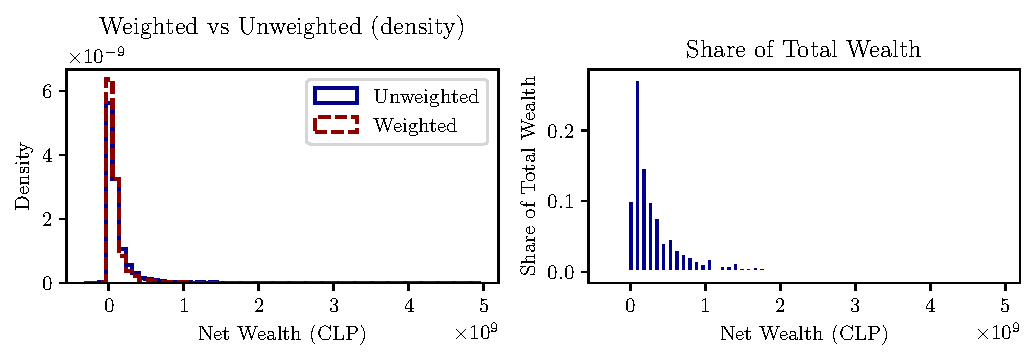
\includegraphics[width=0.95\textwidth]{../../figures/netwealth-efh.pdf}
    \caption{Household Wealth Distribution in Chile (EFH 2021, Survey Weighted)}\label{fig:chilean-pop}
\end{figure}


\paragraph{Measuring Inequality.} Using the distribution above, we calculate percentile wealth shares as defined in Equation \ref{eq:wealth_share}, with households ranked by $W_i$ and weighted by expansion factors $w_i$\footnote{See \texttt{source/shares.py:L5-L35} (\texttt{weighted\_shares}).}. Figure \ref{fig:shares-ineq} reports the baseline survey estimates for the top 1\%, top 10\% and bottom 50\%.
\begin{figure}[H]
    \centering
    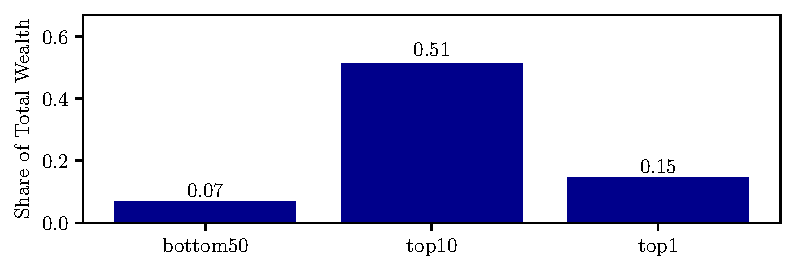
\includegraphics[width=0.85\textwidth]{../../figures/p2/share.pdf}
    \caption{Baseline Wealth Shares in Chile (EFH 2021, No Tail Correction)}\label{fig:shares-ineq}
\end{figure}
These preliminary results show that the top 10\% holds 51\% of total Chilean wealth. However, these shares likely underestimate the top 1\% share because of the differential unit non-response documented in Section~\ref{sec:measuring-wealth}. To address this limitation in the following paragraph we show the results of \citet{vermeulen2018} \footnote{See the whole pipeline in \texttt{notebooks/03\_wealth\_inequality.ipynb} and \texttt{notebooks/04\_vermeulen.ipynb}}.

\paragraph{Forbes Billionaires.} Data on 2021 Chilean billionaires from Forbes is displayed in Figure \ref{fig:billionaires}. We convert USD billions to Chilean pesos using an exchange rate of 759.1 CLP per USD\footnote{See \texttt{source/cleaning.py:L17-L30} (\texttt{convert\_currency}).}.
\begin{figure}[H]
    \centering
    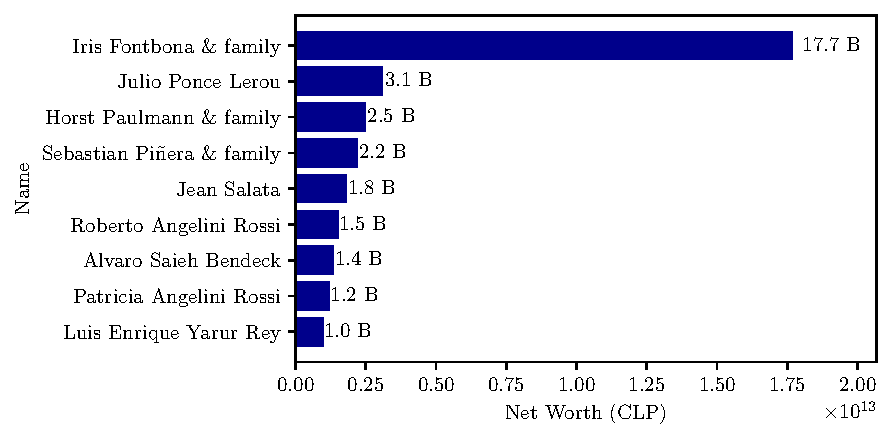
\includegraphics[width=0.90\textwidth]{../../figures/billionaires.pdf}
    \caption{Chilean Billionaires in 2021 (Forbes, Values in CLP)}\label{fig:billionaires}
\end{figure}
Figure \ref{fig:billionaires} is highly skewed: Iris Fontbona holds CLP~17.7~trillion, almost six times the wealth of the remaining eight billionaires in the 2021 Forbes list for Chile.

\paragraph{National Accounts.} Following Equation \ref{eq:wealth_share_na}, we anchor survey aggregates to the December-2021 financial balance for households and non-profit institutions serving households (NPISH)\footnote{File \texttt{data/BDE/CCNN\_CFT\_S14\_AF\_2018.xlsx}, sheet \texttt{Cuadro}, row \texttt{I. Activos Financieros}, December-2021 column; see also \citep{bcentral2021financialaccounts}.}. Let $A^{\text{F,EFH}}=\sum_i w_i A^{\text{F}}_i$ be the survey-weighted financial-asset total and $A^{\text{F,NA}}=426{,}112.5$ billion CLP the macro total; the uprating factor is $\lambda^{\text{F}}=A^{\text{F,NA}}/A^{\text{F,EFH}}$\footnote{See \texttt{source/pareto.py:L83-L107} (\texttt{uprate}).}. We rescale $A^{\text{F}}_i$ by $\lambda^{\text{F}}$ and rebuild $W_i$, so the corrected shares use $W^{\text{NA}}$ as denominator. In 2021 $\lambda^{\text{F}}\approx 0.48$, i.e.\ the survey overstates financial assets relative to the balance-sheet benchmark once pensions are treated separately.

\paragraph{Setting $w_{\min}$ the starting point of the tail.} The cutoff $w_{\min}$ is the wealth level above which power-law behavior is assumed. We set it endogenously as the 99th percentile of the survey-weighted wealth distribution\footnote{See \texttt{source/pareto.py:L131-L147} (\texttt{\_wmin\_from\_percentile}).}, following the survey practice of fitting the tail only at the very top. 

In 2021, $w_{\min}$ ranges from CLP 380--760 million depending on specification, i.e.\ whether we fix it exogenously at USD 0.5m ($\approx$ CLP 380m at 759.1 CLP/USD) or USD 1m ($\approx$ CLP 759m), or set it endogenously as the survey-weighted p99, so we report sensitivity across these three cutoffs. Figure \ref{fig:alpha-sensitivity} shows the estimated tail index falls as the cutoff is lowered: the MLE rises from 1.86 at CLP 380m to 2.53 at the p99, while the regression estimator is stable around 2.13--2.16.
\begin{figure}[H]
    \centering
    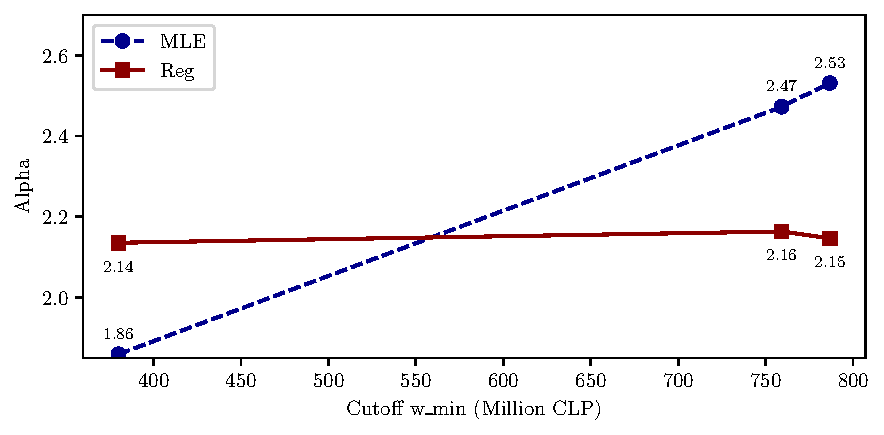
\includegraphics[width=0.85\textwidth]{../../figures/p2/alpha_sensitivity.pdf}
    \caption{Sensitivity of $\hat{\alpha}$ to $w_{\min}$ (MLE vs.\ Regression)}\label{fig:alpha-sensitivity}
\end{figure}

The choice matters because $\hat{\alpha}$ and the corrected top shares move with $w_{\min}$. There is no consensus on an optimal data-driven rule: in practice $w_{\min}$ is chosen by visual inspection of log-log rank plots or goodness-of-fit heuristics \citep[e.g.,][]{clauset2009power,vermeulen2018}, and finding an optimal selector remains an open problem in the literature.

\paragraph{Vermeulen correction.} We fill the gap $[\max(\text{EFH})\approx 4.9\text{b}, \min(\text{Forbes})\approx 987\text{b}]$ with Pareto draws $w = w_{\min}(1-U)^{-1/\hat{\alpha}}$ plus the 9 Forbes records\footnote{See \texttt{source/pareto.py:L148-L187} (\texttt{vermeulen\_correction}).}. As shown in Figure~\ref{fig:pareto_qq}, the MLE slope with $\hat{\alpha}_{\min}\approx 1.85$ (380m cutoff) tracks the empirical points closely, while steeper MLE slopes ($\hat{\alpha}_{\max}\approx 2.53$ at p99) fall below them. By contrast, the Reg panel in the same Figure~\ref{fig:pareto_qq} shows a narrow band ($\approx 2.13$--$2.16$) because $\hat{\alpha}_{\text{Reg}}$ barely moves with $w_{\min}$, so both lines nearly overlap. Figure~\ref{fig:ver_tail} translates this into mass: EFH raw (dashed) truncates at 4.9b, while Vermeulen (solid) bridges the empty gap and extends to 17.7t.

\begin{figure}[H]
    \centering
    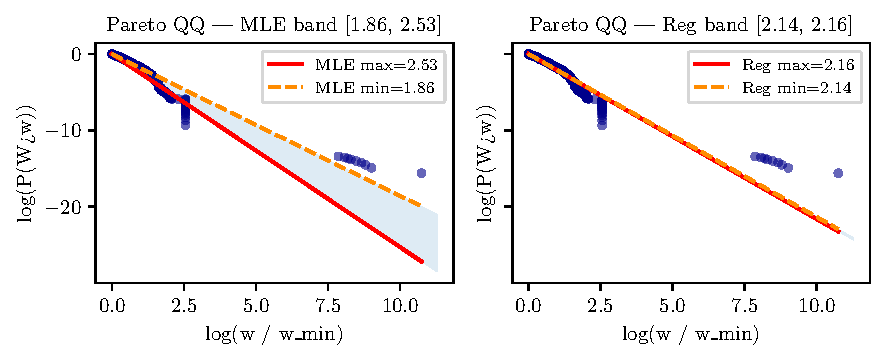
\includegraphics[width=0.95\textwidth]{../../figures/p2/pareto_qq.pdf}
    \caption{Pareto QQ at $w_{\min}=380$m: empirical $\log P(W>w)$ vs.\ $\log(w/w_{\min})$. Left: MLE band, right: Reg band.}\label{fig:pareto_qq}
\end{figure}

\begin{figure}[H]
    \centering
    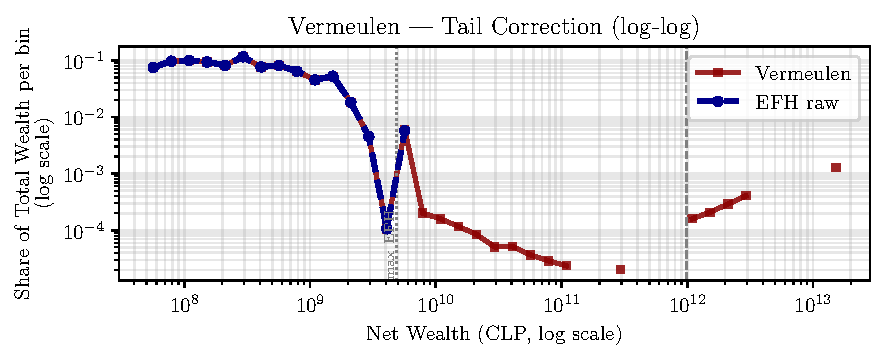
\includegraphics[width=0.95\textwidth]{../../figures/p2/vermeulen_tail.pdf}
    \caption{Tail density (log-log): share per bin, EFH raw vs.\ Vermeulen.}\label{fig:ver_tail}
\end{figure}


\paragraph{Final Comparison.} Table~\ref{tab:shares-corr} compares raw and corrected shares. Both Figure~\ref{fig:ver_tail} and Figure~\ref{fig:wealth-comparison} use $\hat{\alpha}_{\text{MLE}}=1.86$ at $w_{\min}=380$m ($\lambda^{F}\approx 0.48$).
\begin{table}[H]
    \centering
    \caption{Wealth shares: raw vs.\ Vermeulen (380m, MLE $\hat{\alpha}=1.86$)}\label{tab:shares-corr}
    \begin{tabular}{lccc}
        \toprule
        & bottom50 & top10 & top1 \\
        \midrule
        Raw & 6.8\% & 51.4\% & 14.6\% \\
        Corrected & 5.6\% & 53.6\% & 15.8\% \\
        \bottomrule
    \end{tabular}
\end{table}
Correction shifts about 1pp to the top.

\begin{figure}[H]
    \centering
    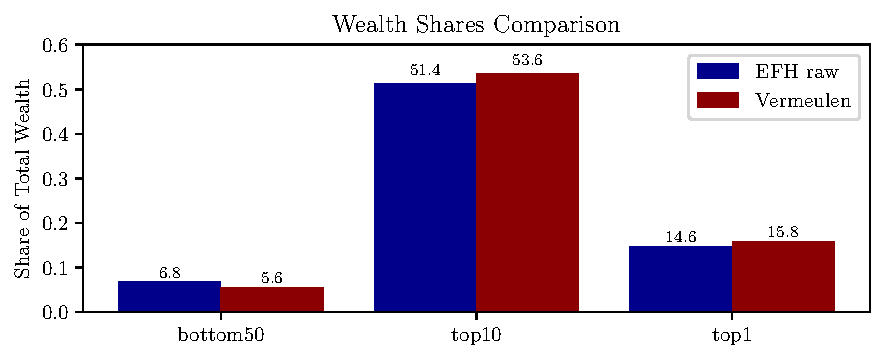
\includegraphics[width=0.95\textwidth]{../../figures/p2/shares_vermeulen.pdf}
    \caption{Wealth shares raw vs.\ Vermeulen-corrected (380m, MLE $\hat{\alpha}=1.86$): bottom50, top10, top1.}\label{fig:wealth-comparison}
\end{figure}

The effect is modest compared to Vermeulen (2018) (e.g.\ Italy +6pp) because $\hat{\alpha}=1.86$ implies a fatter tail than Reg, yet still thin: the Pareto mean $\hat{\alpha}/(\hat{\alpha}-1)\times w_{\min}$ adds little mass beyond 4.9b. Had we used $\hat{\alpha}_{\text{Reg}}=2.15$ at p99, the top 1\% gain would be roughly half, as suggested by the steeper slope in Figure~\ref{fig:pareto_qq}. The counterpart is the bottom 50\% falling from 6.8\% to 5.6\%: fixing the denominator with $W^{\text{NA}}$ while adding top wealth mechanically dilutes the bottom. In short, the survey captures the middle well but misses the extreme right, and the correction size hinges entirely on $\hat{\alpha}$.

\newpage
\section{Moving Beyond Vermeulen: BFM (2022)}\label{sec:bfm-methodology}
%! TEX root = ../main.tex
We previously examined the correction proposed by \citet{vermeulen2018} for differential unit non-response (Section~\ref{sec:measuring-wealth}). The intuition is that household surveys fail to capture billionaires at the extreme right tail. Since this group is small and largely identifiable, observing its wealth allows us to recover the extended Pareto tail. While effective, the method is sensitive to the threshold chosen to define and estimate the tail (see Section~\ref{sec:results}).

In this section, we discuss an alternative data-driven approach proposed by \citet{blanchet2022weight} that does not rely on a parametric Pareto assumption. Due to the lack of tabulated wealth tax data for Chile, we do not apply this correction to wealth inequality but illustrate it for income inequality using the National Socioeconomic Characterization Survey (CASEN) waves 2017 and 2022 \citep{casen2017, casen2022}.

\subsection*{The Blanchet-Flores-Morgan (BFM) Technique}\label{sec:bfm}
\citet{blanchet2022weight} develop a calibration-based method to reconcile survey microdata with tabulated tax data. Unlike \citet{vermeulen2018}, the method does not assume a Pareto tail from an ad hoc cutoff $w_{\min}$. Instead, it endogenously determines a \textit{merging point} $y^{*}$ above which tax data become more reliable than the survey, and then corrects the survey via reweighting and imputation while preserving its demographic structure.

\paragraph{The Merging point}\label{sec:bfm-merging}
Let $f(y)$ and $F(y)$ denote the income density and cumulative distribution, with subscripts $s$ for survey and $t$ for tax tabulations. Define the density ratio and the cumulative ratio as:
\begin{equation}
    \theta(y) = \frac{f_{s}(y)}{f_{t}(y)}, \qquad \Theta(y) = \frac{1-F_{s}(y)}{1-F_{t}(y)}.
    \label{eq:theta-Theta}
\end{equation}
If the survey were representative at income $y$, $\theta(y)=\Theta(y)$. The central assumption in \citet{blanchet2022weight} is that representativeness is constant up to $y^{*}$ and strictly decreasing thereafter, reflecting systematic under-coverage of the rich due to non-response and misreporting. The merging point $y^{*}$ is then defined as the largest income such that the density ratio and the cumulative ratio coincide:
\begin{equation}
    y^{*} = \sup \{ y : \theta(y) = \Theta(y) \}.
    \label{eq:merging-point}
\end{equation}
Below $y^{*}$ the survey is trusted; above $y^{*}$ the tax data dominate. By construction, $y^{*}$ is higher (more conservative) than the quantile-crossing point used in earlier hybrid methods, thereby minimizing unnecessary distortion of the survey \citep[see Appendix~A.3 in][]{blanchet2022weight}. Crucially, to guarantee that such an empirical intersection exists and is analytically unique—both in continuous distributions and across discrete quantile brackets—formal mathematical proofs are provided in Appendix~\ref{app:merging-point-proof}.

\paragraph{Estimation of $y^{*}$.}
The practical problem is to locate $y^{*}$ from tabulated tax data and survey microdata without imposing an arbitrary threshold. We construct a fractal percentile grid with 126 bins: 99 bins of 1~pp covering $0$--$99\%$, followed by $9$ bins of $0.1$~pp for $99$--$99.9\%$, $9$ bins of $0.01$~pp for $99.9$--$99.99\%$, and $9$ bins of $0.001$~pp for $99.99$--$99.999\%$, as shown in Figure~\ref{fig:fractal}. The SII tabulations are interpolated via generalized Pareto interpolation \citep{blanchet2022generalized}\footnote{Implemented in \texttt{source/bfm.py:61-116} (\texttt{interpolate\_tax\_tabulation}), which shells out to R through \texttt{source/gpinter\_bridge.R}; without R and the \texttt{gpinter} package the code falls back to linear interpolation with a warning.} using, for each bracket, the number of taxpayers and mean income. The first SII bracket is exempt ($0$--$13.5$~UTA), so the fiscal CDF is adjusted and evaluated only above the second bracket lower bound $y_2$:
\begin{equation}
F_t(y_2) = 1 - \kappa + \kappa w_1,
\label{eq:ft-y2}
\end{equation}
where $\kappa$ is taxpayers over adult population (fiscal coverage) and $w_1$ is the first-bracket share in the raw SII tabulation. The grid therefore runs over $[F_t(y_2), 1]$.

Figure~\ref{fig:fractal} shows why the binning is called fractal: at each level the $1\%$ tail left unexplained is re-divided by $10$, so resolution grows exactly where non-response is concentrated.

\begin{figure}[H]
    \centering
    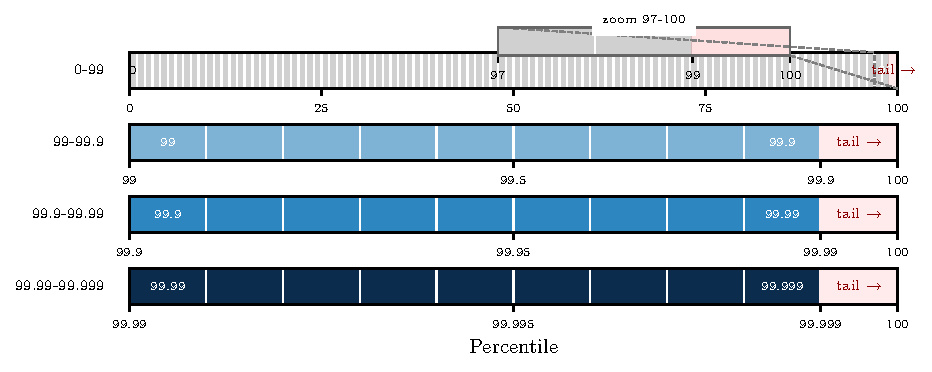
\includegraphics[width=0.85\textwidth]{../../figures/p3/bfm_fractal_bins.pdf}
    \caption{Fractal bins for tax tabulations in \citet{blanchet2022weight}. Each row zooms into the tail (red-hatched) of the row above. The top row covers $0$--$99\%$ with $99$ bins of $1$~pp; subsequent rows split the remaining tail into $9$ bins of $0.1$, $0.01$ and $0.001$~pp, respectively. The inset in the top panel magnifies the $97$--$100\%$ region where the $99\%$ cutoff would otherwise be invisible.}
    \label{fig:fractal}
\end{figure}

Let $d_i$ denote the survey design weight of observation $i$ and $N_s=\sum_{i} d_i$ the survey-weighted population. For bin $k=[y_k,y_{k+1})$ with width $width_k=y_{k+1}-y_k$, let $w_k$ be the tax-data population share of the bin (e.g., $1$~pp, $0.1$~pp) and $\text{share}_{s,k}=\sum_{i: y_i\in bin_k} d_i/N_s$ the corresponding survey share. Histogram densities are $f_{t,k}=w_k/width_k$ and $\tilde{f}_{s,k}=\text{share}_{s,k}/width_k$, so the raw ratio is
\begin{equation*}
\tilde{\theta}_{k}= \frac{\tilde{f}_{s,k}}{f_{t,k}} = \frac{\text{share}_{s,k}}{w_k}= \frac{\sum_{i: y_i \in \text{bin }k} d_i/N_s}{w_k},
\end{equation*}
i.e., the survey share in the bin divided by the tax-data share; $width_k$ cancels but makes explicit that $\tilde{\theta}_k$ compares densities. Because $\tilde{\theta}_{k}$ is noisy, \citet{blanchet2022weight} smooth it via an antitonic (monotonically decreasing) regression:
\begin{equation}
    \min_{\hat{\theta}_{1}\ge \cdots \ge \hat{\theta}_{m}} \sum_{k=1}^{m} w_{k} (\hat{\theta}_{k} - \tilde{\theta}_{k})^{2},
    \label{eq:antitonic}
\end{equation}
where $w_{k}$ is the population share of bin $k$, solved by the Pool Adjacent Violators Algorithm. 

Once $\tilde{\theta}$ is smoothed, the merging point is estimated as the lowest bin $k^{*}$ such that $\hat{\theta}_{k^{*}} < \hat{\Theta}_{k^{*}}$, with fiscal incomes in tabulations interpolated via the generalized Pareto interpolation of \citet{blanchet2022generalized}. $\Theta(y)$ is already stable and can be estimated directly from empirical CDFs:
\begin{equation}
    \hat{\Theta}(y)=\frac{1-\hat{F}_{s}(y)}{1-\hat{F}_{t}(y)}, \quad 
    \hat{F}_{s}(y)=\frac{1}{N_s}\sum_{i=1}^{N_s} d_i\mathbf{1}\{y_i \le y\},
    \label{eq:Theta-hat}
\end{equation}
where $\hat{F}_{t}(y)$ is obtained from the interpolated tax tabulation and $\hat{\Theta}_{k}=\hat{\Theta}(y_k)$ at the lower bound of bin $k$.

\paragraph{Normalization of units.}
Because the SII tabulations count individual taxpayers while CASEN records total household income, the two distributions are not directly comparable. We express both in annual income per adult: each household's income is \texttt{ytotcorh} $\times$ 12 divided by the number of adults aged 20 or older, and the effective weight is the household expansion factor times the number of adults. Without this conversion the household-level survey density cannot be aligned with the individual-level fiscal density.

\paragraph{Reweighting via calibration.}\label{sec:bfm-reweighting}
Given $y^{*}$, the survey is corrected to match tax-data totals above the threshold while preserving representativeness in other dimensions (age, gender, household type). This is achieved through linear calibration \citep{DevilleSarndal1992}, routinely used by statistical agencies. Let $\{(x_{i}, d_{i})\}_{i=1}^{n}$ be the survey sample with $k$-dimensional covariates $x_{i}$ and design weights $d_{i}$, and let $T$ be the vector of known population totals from external sources. Calibrated weights $\{w_{i}\}$ solve:
\begin{equation}
    \min_{\{w_{i}\}} \sum_{i=1}^{n} \frac{(w_{i}-d_{i})^{2}}{d_{i}} \quad \text{s.t.} \quad \sum_{i=1}^{n} w_{i} x_{i} = T, \quad \frac{1}{\alpha} \le \frac{w_{i}}{d_{i}} \le \alpha,
    \label{eq:calibration}
\end{equation}
with truncation $\alpha=5$ to avoid extreme adjustments, followed by a uniform rescaling below and above $y^{*}$ to match exactly the tax-data count above the merging point. Unlike the estimation of $y^{*}$, no shape restriction is imposed on $\theta(y)$ above $y^{*}$; empirical ratios are used directly, including local overestimation due to heaping at round values.

\paragraph{Expanding the support.}
Calibration alone cannot create incomes beyond the survey support $\max(y_{s})$. When tax tabulations extend further, \citet{blanchet2022weight} inflate the sample by splitting each observation $i$ into $k_{i}=[\pi \cdot w_{i}]$ copies with weight $q_{i}=w_{i}/k_{i}$, and assign incomes from the continuous distribution fitted to tax data by generalized Pareto interpolation, preserving the rank of observations. This addresses small-sample bias at the very top, which calibration corrects only asymptotically \citep{DevilleSarndal1992}.

\begin{algorithm}[H]
    \caption{Blanchet-Flores-Morgan (2022) Correction Procedure}\label{alg:bfm}
    \SetAlgoLined
    \KwIn{Survey microdata $\{(y_{i}, d_{i}, x_{i})\}_{i=1}^{N}$; tabulated tax data $\{b_{k}\}_{k=1}^{m}$; calibration totals $T$.}
    \KwOut{Merging point $y^{*}$; calibrated weights $\{w_{i}\}$; augmented sample with corrected shares.}
    \BlankLine
    \tcp{Step 1: Estimate merging point $y^{*}$}
    Interpolate tax tabulations via generalized Pareto; compute $\hat{\Theta}_{k}$ and $\tilde{\theta}_{k}$ per bin; smooth to $\hat{\theta}_{k}$ via antitonic regression \eqref{eq:antitonic}; set $y^{*}$ as first bin with $\hat{\theta}_{k} < \hat{\Theta}_{k}$\;
    \BlankLine
    \tcp{Step 2: Calibration reweighting}
    Solve \eqref{eq:calibration} to obtain $w_{i}$ matching tax-data mass above $y^{*}$ and demographic totals, with truncation $\alpha=5$\;
    \BlankLine
    \tcp{Step 3: Expand support beyond $\max(y_{s})$}
    Duplicate observations as $k_{i}=[\pi w_{i}]$ copies and assign tail incomes from interpolated tax distribution preserving ranks\;
    \BlankLine
    \tcp{Step 4: Recompute inequality indicators}
    Compute corrected top shares and Gini on augmented sample; compare with survey-only baseline\;
\end{algorithm}

Unlike \citet{vermeulen2018}, the BFM procedure is fully data-driven, preserves the joint distribution of income and covariates, guarantees continuity of the density at $y^{*}$, and does not require choosing $w_{\min}$ by visual inspection. Its cost is the need for detailed tabulated tax data covering a sizable share of the population, which is available for income in Chile (SII tabulations) but not for wealth, motivating our application to CASEN income in the next subsection.

\subsection{Data}\label{sec:bfm-data}
We illustrate BFM on income using the National Socioeconomic Characterization Survey (CASEN) for 2017 and 2022 \citep{casen2017, casen2022} and tabulated tax data from the Chilean Internal Revenue Service (SII) \citep[see][for tabulation details]{sii2024personas}. The CASEN microdata are person-level with household identifiers and expansion factors\footnote{See \texttt{source/casen.py:11-28} (\texttt{INCOME\_COLS}, \texttt{load\_casen}) and \texttt{source/casen.py:92-108} (\texttt{to\_household}), plus \texttt{notebooks/05\_data\_exploration.ipynb}; loading uses \texttt{convert\_categoricals=False} to avoid duplicate labels in \texttt{rama4\_sub\_rev3}.}. At the person level $N=216{,}439$ (2017) and $N=202{,}231$ (2022); collapsing to one row per household yields $N_{hh}=70{,}948$ (2017) and $72{,}053$ (2022) with total household income corrected for non-response\footnote{See \texttt{source/casen.py:29-91} (\texttt{income\_overview}, \texttt{summarize\_income}); missingness is $0\%$ for total household income in 2017 and $0.06\%$ in 2022, versus $31$--$44\%$ for uncorrected autonomous income, motivating the choice of total household income; household-level weighted median is CLP~$0.80$M (2017) and $1.11$M (2022).}. We use total household income with survey weights for BFM; per-capita total income is retained for robustness. Household-level data for replication are saved to the processed CASEN household files in \texttt{data/processed}\footnote{See \texttt{notebooks/05\_data\_exploration.ipynb}, Sec.~6 (\texttt{to\_household}, \texttt{OUTPUTDATA}).}. Figure~\ref{fig:casen-income} displays the weighted household income distributions (log scale) and Figure~\ref{fig:casen-lorenz} overlays the corresponding Lorenz curves for 2017 and 2022.
\begin{figure}[H]
    \centering
    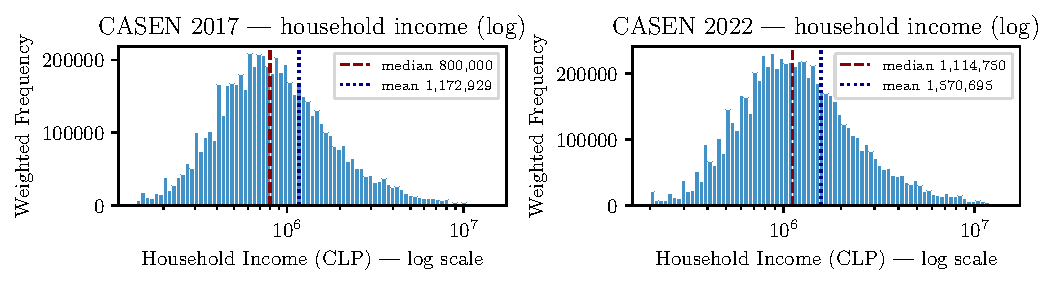
\includegraphics[width=0.85\textwidth]{../../figures/p3/casen_income_dist.pdf}
    \caption{Household income distribution (CASEN, total household income, log scale). Weighted histograms for 2017 and 2022 at household level. Vertical lines mark weighted mean (dotted) and median (dashed). Both years are right-skewed; 2022 shifts right (higher mean/median) but retains a heavy tail. This is the survey density $f_s$ that BFM will compare to $f_t$ from SII tabulations.}
    \label{fig:casen-income}
\end{figure}

\begin{figure}[H]
    \centering
    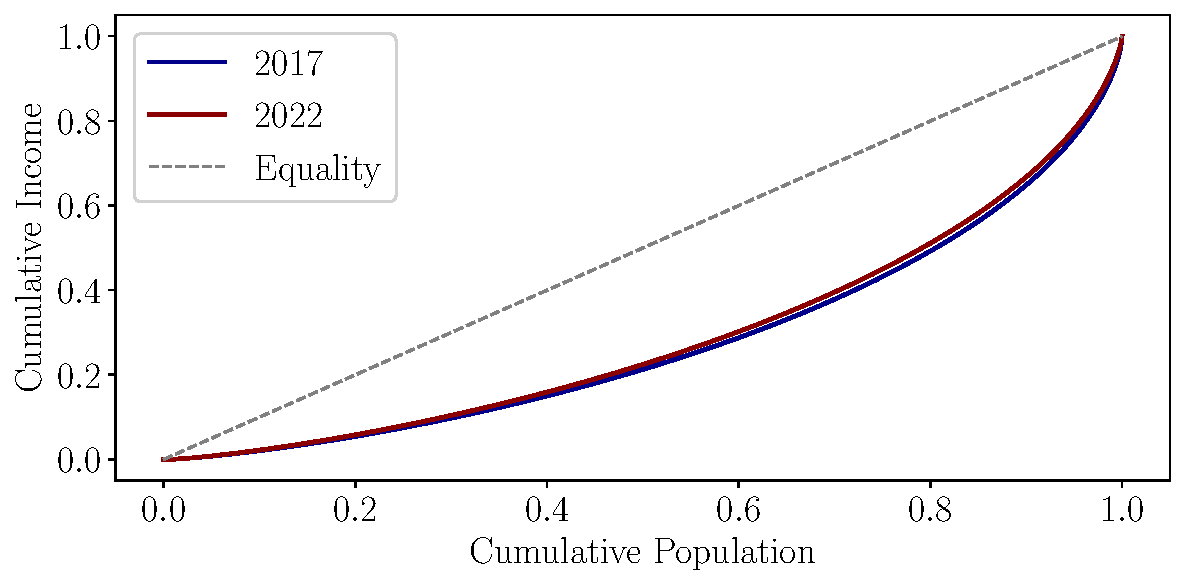
\includegraphics[width=0.60\textwidth]{../../figures/p3/casen_lorenz.pdf}
    \caption{Lorenz curves overlaid (CASEN household income). Cumulative population (weighted) vs.\ cumulative income for 2017 (blue) and 2022 (red), with the $45^{\circ}$ equality line (gray dashed). Proximity of the two curves indicates little change in overall inequality; the gap to the diagonal reflects concentration at the top that motivates the BFM correction.}
    \label{fig:casen-lorenz}
\end{figure}
Tax tabulations are from the SII annual file on natural persons (2005--2024, updated Oct~2025) which reports, by UTA bracket, the number of taxpayers and total income (in MM~CLP) for Global Complementary Tax, Second Category, and Consolidated totals\footnote{See \texttt{source/sii.py:10-118} (\texttt{load\_sii\_pub\_total}, \texttt{sii\_for\_at}) for parsing the double header (rows~6--7) and \texttt{notebooks/05\_data\_exploration.ipynb}, Sec.~5.}. For BFM we use the Consolidated block. The 2020 reform added a top bracket, so the count rises from 7 brackets in 2017 to 8 in 2022, with top brackets \textit{More than 120 UTA (Rate 35\%)} in 2017 and \textit{More than 310 UTA (Rate 40\%)} in 2022; amounts are in MM~CLP at Dec.~31 of each commercial year. Figure~\ref{fig:sii-comparison} compares the Consolidated tabulations by bracket for the two years.
\begin{figure}[H]
    \centering
    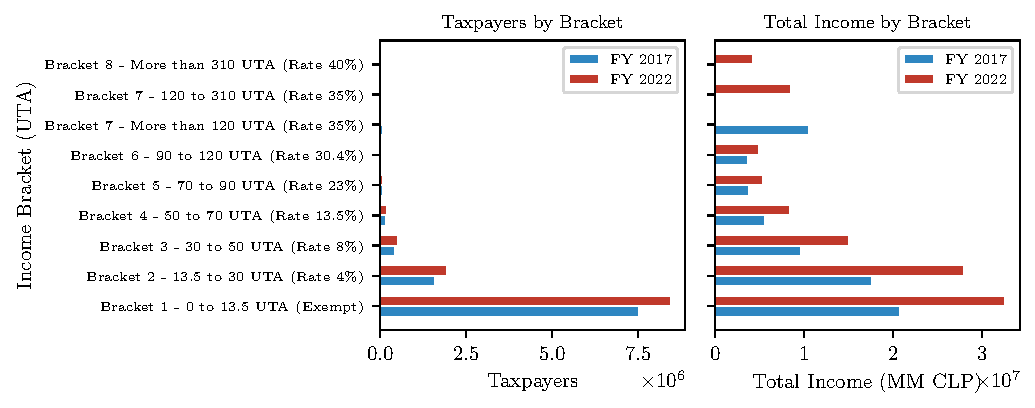
\includegraphics[width=0.95\textwidth]{../../figures/p3/sii_brackets_comparison.pdf}
    \caption{SII tax tabulations (Consolidated) by UTA bracket: 2017 vs.\ 2022 (commercial years, i.e., AT 2018 vs.\ AT 2023). Left: number of taxpayers; right: total income (MM~CLP) per bracket. Bracket labels are translated from Spanish and decimal commas converted to dots; grouping handles the reform-induced change from 7 to 8 brackets (outer join, missing brackets set to 0). This is the fiscal density $f_t$ used to estimate $\tilde{\theta}_k$ and $\hat{\Theta}_k$.}
    \label{fig:sii-comparison}
\end{figure}

\subsection{Results}

Table~\ref{tab:bfm-shares} reports top income shares computed on annual income per adult. The raw CASEN survey understates top incomes relative to the SII tabulations; BFM calibration raises the top-1\% share from 9.17\% to 13.56\% in 2017 and from 7.86\% to 9.40\% in 2022 under the default clip $\alpha=5$. Expanding the support beyond the survey maximum adds a further 0.86~pp in 2017 and 0.36~pp in 2022. In 2022 the required calibration factor exceeds the $\alpha=5$ clip; relaxing it to $\alpha\ge10$ raises the top-1\% share to 10.03\% and, with expansion, to 10.19\%.

\begin{table}[H]
\centering
\caption{Top income shares under BFM correction, annual income per adult (\% of total income)}
\label{tab:bfm-shares}
\small
\begin{tabular}{lcccccc}
\toprule
 & \multicolumn{3}{c}{2017} & \multicolumn{3}{c}{2022} \\
\cmidrule(lr){2-4} \cmidrule(lr){5-7}
Method & Top 10\% & Top 5\% & Top 1\% & Top 10\% & Top 5\% & Top 1\% \\
\midrule
Raw survey & 35.91 & 24.58 & 9.17 & 34.11 & 22.70 & 7.86 \\
BFM calibrated ($\alpha=5$) & 40.16 & 29.27 & 13.56 & 35.43 & 24.12 & 9.40 \\
BFM + support expansion & 40.75 & 29.96 & 14.42 & 35.69 & 24.42 & 9.76 \\
\midrule
2022, $\alpha\ge 10$ & --- & --- & --- & 35.97 & --- & 10.03 \\
2022, $\alpha\ge 10$ + expansion & --- & --- & --- & --- & --- & 10.19 \\
\bottomrule
\end{tabular}
\end{table}

Table~\ref{tab:bfm-params} reports the merging point and calibration diagnostics. Fiscal coverage $\kappa$ is 0.736 in 2017 and 0.763 in 2022. The exempt first bracket shifts the effective start of the fiscal CDF to $F_t(y_2)=0.819$ and 0.804, leaving 45 and 46 bins above $y_2$ in which to search for the merging point. The resulting $y^{*}$ is 68.03~M CLP per year ($\sim$121~UTA) in 2017 and 190.0~M CLP per year ($\sim$271~UTA) in 2022; only 12 survey observations lie above the 2022 threshold.

\begin{table}[H]
\centering
\caption{BFM calibration parameters and merging point}
\label{tab:bfm-params}
\small
\begin{tabular}{lcc}
\toprule
Parameter & 2017 & 2022 \\
\midrule
$y^{*}$ (M CLP/year) & 68.03 ($\sim$121 UTA) & 190.0 ($\sim$271 UTA) \\
$\kappa$ (taxpayer coverage) & 0.736 & 0.763 \\
$F_t(y_2)$ & 0.819 & 0.804 \\
Grid bins used & 45 & 46 \\
Observations above $y^{*}$ & 111 & 12 \\
\bottomrule
\end{tabular}
\end{table}

\begin{figure}[H]
    \centering
    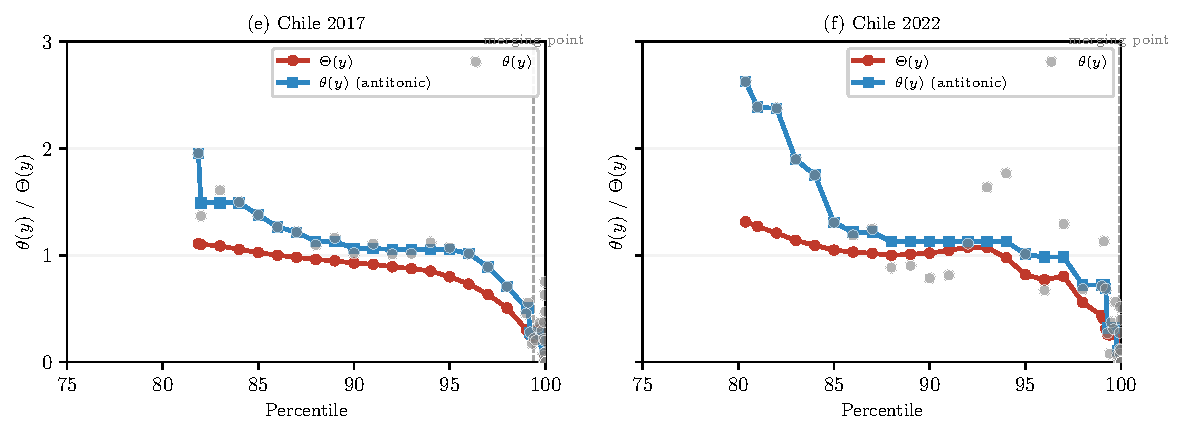
\includegraphics[width=0.95\textwidth]{../../figures/p3/bfm_theta_Theta_real.pdf}
    \caption{BFM empirical diagnostic curves with upper-tail zoom: marginal vs.\ cumulative representativeness ratios for Chile (2017 and 2022). Raw density ratio $\tilde{\theta}(y)$ per fractal bin (gray dots), antitonic isotonic regression $\hat{\theta}(y)$ (blue line with squares), and cumulative ratio $\hat{\Theta}(y)$ (red line with circles). The main axes display the overall trajectory across the upper distribution ($P \ge 75\%$). The inset axes zoom in on the extreme right tail ($P \ge 98\%$), clearly resolving the crossing of $\hat{\theta}(y)$ and $\hat{\Theta}(y)$ at the endogenous merging point $y^*$ (marked by the dashed gray vertical line and labeled percentile). Panel (e) depicts commercial year 2017 ($y^* = 68.03$~M CLP/year, $P99.40$, 111 observations above $y^*$); Panel (f) depicts commercial year 2022 ($y^* = 190.0$~M CLP/year, $P99.90$, 12 observations above $y^*$).}
    \label{fig:bfm-theta-Theta}
\end{figure}

Figure~\ref{fig:bfm-theta-Theta} plots the empirical trajectory of $\tilde{\theta}(y)$, $\hat{\theta}(y)$, and $\hat{\Theta}(y)$ across the upper percentile distribution for 2017 and 2022, directly replicating the diagnostic specification of \citet[][Figure~6e]{blanchet2022weight}. The raw density ratio $\tilde{\theta}(y)$ (gray dots) exhibits substantial sampling dispersion and local heaping around round income values. However, its antitonic PAVA smoothing $\hat{\theta}(y)$ (blue line with squares) displays a strictly non-increasing profile in the upper tail, empirically corroborating the theoretical monotonicity conditions established in Appendix~\ref{app:merging-point-proof}. The cumulative ratio $\hat{\Theta}(y)$ (red line with circles) remains remarkably stable near unity throughout the domain. 

Comparing the two panels highlights significant structural differences across survey waves:
\begin{itemize}
    \item \textbf{Commercial Year 2017 (Panel~e):} The marginal representativeness rate $\hat{\theta}(y)$ tracks the tax density closely across the 82nd to 96th percentiles ($\hat{\theta} \approx 1.0$--$1.2$), indicating high survey fidelity across the upper-middle class. Above the 98th percentile, $\hat{\theta}(y)$ declines sharply and crosses below $\hat{\Theta}(y)$ at $y^* = 68.03$~M CLP/year ($\sim$121~UTA, approximately P99.4). Because 111 survey households lie above this cutoff, the tail calibration is empirically well-supported and stable, and the required calibration factor $(1 - F_t(y^*))/(1 - F_s(y^*)) = 3.78$ falls safely below the $\alpha = 5$ truncation clip.
    \item \textbf{Commercial Year 2022 (Panel~f):} In contrast, $\hat{\theta}(y)$ starts considerably higher in the lower-tax brackets ($\sim 2.6$ near P80), reflecting substantial post-pandemic nominal income growth and high labor informality. It remains elevated ($\hat{\theta} \approx 1.1$) across P86--P94, and crosses $\hat{\Theta}(y)$ only at an extreme threshold of $y^* = 190.0$~M CLP/year ($\sim$271~UTA, P99.8). This high threshold leaves merely 12 survey households above $y^*$, virtually exhausting the survey sample in the extreme tail. As a consequence, the required calibration factor surges to $6.69$, hitting the $\alpha = 5$ truncation constraint (Table~\ref{tab:bfm-sens-factor}) and underscoring the critical necessity of support expansion to avoid downward bias in top wealth/income shares.
\end{itemize}

\paragraph{Sensitivity.}
Table~\ref{tab:bfm-sens-kappa} shows how the top-1\% share and the merging point vary with assumed fiscal coverage $\kappa$. In 2017 the estimated top-1\% share rises monotonically from 10.93\% to 13.56\% as $\kappa$ moves from 0.40 to the estimated 0.736; $y^{*}$ falls from 70.94~M to 66.37~M CLP and then returns to 68.03~M CLP at the estimated $\kappa$. In 2022 the share is flat at 9.40\% for $\kappa\ge0.50$ because the $\alpha=5$ clip is already binding.

\begin{table}[H]
\centering
\caption{Sensitivity to fiscal coverage $\kappa$}
\label{tab:bfm-sens-kappa}
\small
\begin{tabular}{lccccc}
\toprule
$\kappa$ & 0.40 & 0.50 & 0.60 & 0.70 & Estimated \\
\midrule
2017 top 1\% & 10.93 & 11.74 & 12.61 & 13.41 & 13.56 \\
2017 $y^{*}$ (M CLP) & 70.94 & 68.68 & 67.29 & 66.37 & 68.03 \\
2022 top 1\% & 9.04 & 9.40 & 9.40 & 9.40 & 9.40 \\
\bottomrule
\end{tabular}
\end{table}

The required calibration factor $(1-F_t(y^{*}))/(1-F_s(y^{*}))$ is 3.78 in 2017 and 6.69 in 2022 (Table~\ref{tab:bfm-sens-factor}). In 2017 this factor does not hit the $\alpha=5$ clip, so the calibrated results are invariant to the clip. In 2022 the required factor exceeds 5; the clip truncates the adjustment and understates the top-1\% share by roughly 0.8~pp relative to the converged value of 10.19\% obtained with $\alpha\ge10$ and support expansion.

\begin{table}[H]
\centering
\caption{Sensitivity to calibration factor}
\label{tab:bfm-sens-factor}
\small
\begin{tabular}{lcc}
\toprule
 & 2017 & 2022 \\
\midrule
Required factor $(1-F_t(y^{*}))/(1-F_s(y^{*}))$ & 3.78 & 6.69 \\
Hits $\alpha=5$ clip? & No & Yes \\
Implied bias if clipped ($\alpha=5$) & --- & $\sim -0.8$~pp top 1\% \\
Converged top 1\% ($\alpha\ge10$ + expansion) & --- & 10.19 \\
\bottomrule
\end{tabular}
\end{table}

\paragraph{Notes for the reader.}
Three caveats qualify these results. (i) The public SII file \texttt{PUB\_Total.xlsb} reports only 7--8 brackets (7 in 2017--2019, 8 thereafter, sheets \texttt{Datos} and \texttt{Notas}), with no decile breakdown. The top-1\% threshold is therefore identified directly from the tabulation only in 2017; in later years it must be inferred from the interpolated tail. (ii) The 2022 merging point rests on only 12 survey observations above $y^{*}$, so the tail is thin and the correction relies heavily on the interpolation. (iii) The support expansion implemented here is a quantile mapping that preserves ranks and total mass; it is not a literal duplication of observations.

\newpage
\section{Conclusions}\label{sec:conclusions}
%! TEX root = ../main.tex
This report has investigated three interrelated dimensions of economic inequality and intergenerational transmission in Chile, combining microeconometric estimation, survey microdata, administrative tax records, and external wealth registries. Together, the findings provide a comprehensive empirical assessment of persistence and concentration while highlighting the critical role of modern econometric corrections.

\subsection*{Summary of Empirical Findings}

First, our replication and extension of \citet{nunez2010mobility} in Section~\ref{sec:intergenerational-mobility} demonstrates that Chile exhibits substantial intergenerational income persistence. The estimated TSTSLS income elasticities range between 0.61 (conditioning on paternal schooling and occupation) and 0.83 (schooling only), confirming that parental background exerts a first-order influence on offspring earnings. Beyond the baseline replication, our extensions reveal that labor informality introduces significant heterogeneity into the transmission mechanism: sons contributing to the pension system display substantially higher rank--rank persistence (slope of 0.320) than informal workers (0.295; Spearman rank correlation of 0.250). Furthermore, our multiple imputation sensitivity analysis underscores that the assumed correlation between paternal and filial unobservables critically shapes estimated persistence, demonstrating that social security affiliation is an essential institutional mediator of mobility in developing economies.

Second, our analysis of household wealth inequality in Section~\ref{sec:wealth-inequality} highlights the pervasive limitations of self-reported survey data. Standard surveys like the EFH suffer from unit non-response at the extreme right tail, and the presence of negative net worth ($L_i > A_i$) distorts synthetic inequality metrics such as the Gini coefficient, mathematically breaking its standard axiomatic bounds (Appendix~\ref{app:gini-negative}). By implementing the semi-parametric Pareto tail correction of \citet{vermeulen2018} augmented with the \textit{Forbes World's Billionaires} census and benchmarking aggregates to National Accounts, we demonstrate that top wealth shares in Chile are substantially higher than raw survey tabulations indicate. Microfoundations of multiplicative accumulation and scale-dependent returns (Appendix~\ref{app:pareto-foundations}) justify the power-law tail, showing that capital concentration cannot be captured without accounting for ultra-high-net-worth individuals.

Third, in Section~\ref{sec:bfm-methodology}, we evaluated the frontier non-parametric calibration framework of \citet{blanchet2022weight} (BFM) using CASEN 2017 and 2022 microdata combined with tabulated administrative tax records from the SII. In contrast to parametric Pareto adjustments that rely on an exogenously chosen cutoff $w_{\min}$, the BFM approach endogenously locates the survey-tax merging point $y^*$ where marginal representativeness matches cumulative coverage. We provided formal analytical proofs establishing the sufficient conditions for the existence and uniqueness of this merging point in both continuous and discrete settings (Appendix~\ref{app:merging-point-proof}). Empirically, BFM calibration shifts substantial mass to the upper decile, increasing the top-1\% income share by over 4.4~pp in 2017 (from 9.17\% to 13.56\%, and 14.42\% with support expansion). For 2022, post-pandemic nominal income growth and tax bracket restructuring pushed the merging point to an extreme threshold of $y^* \approx 190.0$~M CLP/year (leaving only 12 survey observations above $y^*$), illustrating how calibration constraints bind when survey coverage is thin and proving the necessity of rank-preserving support expansion.

\subsection*{Methodological and Policy Implications}

The unified takeaway from this investigation is that no single empirical source is sufficient for inequality and mobility measurement. Household surveys remain indispensable for observing demographic attributes, informal labor, and the bottom half of the distribution, but fail systematically in the tail due to non-response and under-reporting. Conversely, administrative tax records provide comprehensive tracking of formal capital and labor at the top, but exclude informal workers and low-income exempt individuals. 

Rigorous distributional analysis and effective public finance design---such as evaluating wealth taxes, progressive income reforms, and social safety nets---require hybrid methodologies that combine administrative registries with representative surveys under explicit calibration principles. The open-source empirical toolkit developed in this project provides a modular, reproducible foundation for implementing these state-of-the-art corrections in Chile and across developing contexts.



% =========================

\newpage
\bibliographystyle{plainnat}
\bibliography{references}

\newpage
\appendix
%! TEX root = ../main.tex
\section{Mathematical Consequences of Negative Net Wealth on the Gini Coefficient}\label{app:gini-negative}

The standard Gini coefficient was originally formulated for non-negative income distributions ($y_i \ge 0$). When applied to net wealth ($W_i \in \mathbb{R}$), where liabilities can exceed assets ($L_i > A_i \implies W_i < 0$), several desirable axiomatic properties of inequality measurement break down \citep{chen1982relative,raffinetti2015does}.

\subsection*{1. Standard Definition of the Gini Index}
For a finite population of size $N$ with wealth vector $(W_1, \dots, W_N)$ sorted in non-decreasing order ($W_1 \le W_2 \le \dots \le W_N$) and mean wealth $\bar{W} = \frac{1}{N}\sum_{i=1}^N W_i$, the Gini coefficient is defined through relative mean difference as:
\begin{equation}
    G = \frac{\sum_{i=1}^N \sum_{j=1}^N |W_i - W_j|}{2 N^2 \bar{W}} = \frac{2 \sum_{i=1}^N i W_i - (N + 1)\sum_{i=1}^N W_i}{N \sum_{i=1}^N W_i}.
    \label{eq:gini_def}
\end{equation}

\subsection*{2. Failure of the Boundedness Axiom ($G \in [0, 1]$)}
Under non-negative values ($W_i \ge 0$ for all $i$ and $\bar{W} > 0$), $G$ is strictly bounded in $[0, 1]$:
\begin{itemize}
    \item $G = 0$ corresponds to perfect equality ($W_1 = W_2 = \dots = W_N = \bar{W}$).
    \item $G = \frac{N-1}{N} \to 1$ corresponds to extreme concentration ($W_1 = \dots = W_{N-1} = 0$, $W_N = N\bar{W}$).
\end{itemize}

However, when negative net wealth is present, the mean wealth in the denominator $\bar{W}$ is compressed downwards because negative and positive balances offset each other, while the numerator $\sum_{i,j} |W_i - W_j|$ strictly increases (as pairwise absolute distances between heavily indebted individuals and wealthy individuals become larger).

\paragraph{Mathematical Proof that $G > 1$:}
Consider a simple stylized 3-agent economy with net wealth values:
\[
    W_1 = -d \quad (d > 0), \quad W_2 = 0, \quad W_3 = M \quad (M > d).
\]
Total wealth is $\sum_{i=1}^3 W_i = M - d > 0$, and mean wealth is $\bar{W} = \frac{M - d}{3}$. Computing the sum of all pairwise absolute differences:
\begin{align*}
    \sum_{i=1}^3 \sum_{j=1}^3 |W_i - W_j| &= 2 \left( |W_1 - W_2| + |W_1 - W_3| + |W_2 - W_3| \right) \\
    &= 2 \left( d + (M + d) + M \right) = 4M + 4d.
\end{align*}
Applying the Gini definition \eqref{eq:gini_def}:
\begin{equation}
    G = \frac{4(M + d)}{2 \cdot 3^2 \cdot \left(\frac{M - d}{3}\right)} = \frac{4(M + d)}{6(M - d)} = \frac{2(M + d)}{3(M - d)}.
\end{equation}
For any case where $d > \frac{M}{5}$ (with $M > d$):
\[
    2(M + d) > 3(M - d) \iff 2M + 2d > 3M - 3d \iff 5d > M \iff G > 1.
\]
As aggregate net wealth approaches zero from above ($\bar{W} \to 0^+$, i.e., $d \to M^-$):
\begin{equation}
    \lim_{\bar{W} \to 0^+} G = +\infty.
\end{equation}
If $\bar{W} < 0$, the denominator becomes negative, rendering $G < 0$ and completely invalidating the geometric and economic interpretation of the Lorenz curve.

\subsection*{3. Violation of Subgroup Decomposability and Monotonicity}
In addition to the loss of bounds:
\begin{itemize}
    \item \textbf{Non-Monotonicity with Respect to Debt Shocks:} Transferring wealth from an indebted individual to a poorer indebted individual (or taking on further debt) can paradoxically lower $G$ if it compresses the denominator faster than the numerator.
    \item \textbf{Failure of Scale Invariance:} While multiplying all wealth by a positive constant $\lambda > 0$ preserves $G$, shifting all wealth by an additive debt transfer fundamentally distorts the ordering, and standard decompositions into between-group and within-group inequality fail because Lorenz curves can cross the horizontal axis and dip substantially below zero.
\end{itemize}
These mathematical instabilities explain why the empirical wealth literature \citep[e.g.,][]{vermeulen2018,oecd2013wealth} predominantly relies on percentile wealth shares rather than synthetic Gini indices.


\newpage

\section{Microfoundations of the Power-Law Tail in Wealth}\label{app:pareto-foundations}

A classic question in the economics of inequality is why wealth distributions consistently exhibit a Pareto (power-law) right tail, $P(W > w) \propto w^{-\alpha}$, rather than standard thin-tailed alternatives such as the log-normal or exponential distributions \citep{gabaix2009power,benhabib2018skewed}. The theoretical justification rests on three foundational mechanisms:

\subsection*{1. Multiplicative Wealth Accumulation and Gibrat's Law}
Consider the dynamic wealth accumulation process of household $i$ across discrete periods $t$:
\begin{equation}
    W_{i, t+1} = (1 + r_{i, t}) W_{i, t} + Y_{i, t} - C_{i, t},
    \label{eq:wealth_accumulation}
\end{equation}
where $r_{i, t}$ denotes the stochastic net rate of return on capital, $Y_{i, t}$ is labor income, and $C_{i, t}$ represents consumption. For households situated in the middle or lower strata of the distribution, labor earnings ($Y_{i, t}$) and essential consumption expenditures ($C_{i, t}$) dominate the evolution of net worth. Consequently, additive shocks prevail, generating an empirical distribution that closely approximates a log-normal profile with non-negligible mass at zero and negative net wealth.

In contrast, for individuals in the upper tail ($W_{i, t} \ge w_{\min}$), accumulated wealth dwarfs labor income and living expenses ($W_{i, t} \gg Y_{i, t} - C_{i, t}$). Under these conditions, the accumulation equation simplifies to an essentially multiplicative stochastic process (Gibrat's law of proportionate growth):
\begin{equation}
    W_{i, t+1} \approx (1 + r_{i, t}) W_{i, t}.
\end{equation}
As demonstrated in the seminal work of \citet{champernowne1953model} and modern random growth theories \citep{gabaix2009power}, the combination of multiplicative random shocks with a lower reflective boundary (or demographic turnover through birth-death generational processes) yields a unique stationary distribution that converges asymptotically to a power law in the tail:
\begin{equation}
    \lim_{w \to \infty} P(W > w) = c \cdot w^{-\alpha},
\end{equation}
where the tail index $\alpha$ is uniquely determined by the balance between the drift and variance of capital returns relative to the discount rate and generational mortality.

\subsection*{2. Scale-Dependent Returns and Portfolio Heterogeneity}
In reality, the rate of return on capital $r_{i, t}$ is not independent of scale. Empirical evidence shows that ultra-high-net-worth individuals systematically earn higher and more volatile average returns on wealth \citep{fagereng2020heterogeneity}. This return premium arises from:
\begin{itemize}
    \item Greater capacity to absorb liquidity risk through substantial allocations to private equity, real estate development, and venture capital.
    \item Lower relative risk aversion and cheaper access to credit.
    \item Significant economies of scale in professional wealth management and exclusive financial information.
\end{itemize}
When expected returns scale positively with wealth, the right tail fattens further, reinforcing the empirical validity of the Pareto specification.

\subsection*{3. Scale Invariance and the Self-Similar Property}
A hallmark feature of the Pareto tail is scale invariance:
\begin{equation}
    \frac{P(W > k \cdot w)}{P(W > w)} = k^{-\alpha}, \quad \forall k > 1.
\end{equation}
Economically, this implies a fractal-like hierarchy: the distribution of wealth among the top 0.1\% relative to the top 1\% exhibits the exact same structural concentration as that of the top 0.01\% relative to the top 0.1\%. This scale-free regularity is consistently corroborated by external billionaire rankings (e.g., Forbes) and tax registry administrative records across diverse economies.

Hence, the semi-parametric methodology proposed by \citet{vermeulen2018} partitions the domain at $w_{\min}$: the empirical survey weights capture the heterogeneous lower and middle portions of the population, while the parametric Pareto distribution accurately restores the fat upper tail where multiplicative accumulation governs.


\newpage

\section{Sufficient Conditions for the Existence and Uniqueness of the Merging Point}\label{app:merging-point-proof}

\begin{center}
    \small
    \textbf{Authors:} Sebastián Rivera\textsuperscript{*} (Lead Author), Cristóbal Donoso, and Cristian Valenzuela \\
    \vspace{0.1em}
    \footnotesize{\textsuperscript{*}Primary theoretical derivation and analytical proof.}
\end{center}
\vspace{0.8em}

\subsection*{1. Introduction and Theoretical Framework}

Accurately measuring income inequality requires combining multiple data sources to overcome the inherent limitations of any single survey instrument. Household surveys, traditionally relied upon for distributional analysis, suffer from a systematic distortion known as \textit{the missing tail problem}. As income rises, the probability of an individual responding to the survey drops monotonically (differential unit non-response), and respondents in the upper deciles systematically under-report their true income, particularly from capital and business assets \citep{deaton2005measuring}.

Conversely, administrative tax records capture the upper tail with high precision and coverage. However, they fail to adequately represent low- and middle-income strata due to legal tax exemption thresholds and widespread labor informality in developing economies. To resolve this structural discrepancy, \citet{blanchet2022weight} developed a non-parametric calibration framework that preserves the survey structure in the lower and middle distribution while transitioning to administrative tax records in the upper tail.

The core methodological challenge lies in identifying an objective income threshold above which the survey distribution should be discarded in favor of tax records. This cutoff is termed the \textit{merging point} ($y^*$). In \citet{blanchet2022weight}, this point is determined endogenously where the relative density (marginal representativeness rate) equals the relative cumulative distribution between both sources. To ensure that this empirical calibration is well-defined and robust, it is essential to establish analytical conditions guaranteeing that the merging point exists and is strictly unique.

In this appendix, we formalize the sufficient conditions for the existence and uniqueness of the merging point in both continuous income distributions and discrete quantile tabulations (such as generalized Pareto curves). The theoretical derivations rely on three foundational empirical premises:
\begin{enumerate}
    \item \textbf{Upper-tail under-representation and monotonicity:} In high-income strata, the survey captures progressively fewer individuals relative to tax registers ($\theta'(y) < 0$ and $\theta(y) < 1$).
    \item \textbf{Initial over-representation anchoring:} Because surveys encompass informal and untaxed earnings, they capture more population than tax registers in the lower and middle strata ($\theta(y^*) \ge \Theta(y^*)$).
    \item \textbf{Population conservation:} Integrating over the entire distribution, both sources converge to 100\% of the target population ($\lim_{y \to \infty} \Theta(y) = 1$). Any initial excess representation in the survey must asymptotically be offset by an upper-tail deficit.
\end{enumerate}

\subsection*{2. The Continuous Case}

Let income $y$ follow a continuous distribution over support $[y_{\min}, \infty)$.

\begin{definition}[Continuous Representativeness Dynamics]
Let $f_X$ and $F_X$ denote the probability density function (PDF) and cumulative distribution function (CDF) of the survey distribution, respectively. Let $f_Y$ and $F_Y$ denote the corresponding PDF and CDF from administrative tax records. We define two key metrics:
\begin{itemize}
    \item \textbf{Marginal representativeness rate:} $\theta(y) = \frac{f_X(y)}{f_Y(y)}$.
    \item \textbf{Cumulative representativeness rate:} $\Theta(y) = \frac{F_X(y)}{F_Y(y)}$.
\end{itemize}
\end{definition}

The trajectory of cumulative representativeness $\Theta(y)$ across the income domain is governed by an ordinary differential equation derived via the quotient rule:
\begin{align*}
    \frac{\mathrm{d}}{\mathrm{d}y}\Theta(y) &= \frac{\mathrm{d}}{\mathrm{d}y}\left( \frac{F_X(y)}{F_Y(y)} \right) = \frac{F_X'(y)F_Y(y) - F_X(y)F_Y'(y)}{[F_Y(y)]^2} = \frac{f_X(y)F_Y(y) - F_X(y)f_Y(y)}{[F_Y(y)]^2}.
\end{align*}
Factoring out $\frac{f_Y(y)}{F_Y(y)}$ on the right-hand side:
\begin{align*}
    \frac{\mathrm{d}}{\mathrm{d}y}\Theta(y) &= \frac{f_Y(y)}{F_Y(y)} \left[ \frac{f_X(y)F_Y(y)}{f_Y(y)F_Y(y)} - \frac{F_X(y)}{F_Y(y)} \right] = \frac{f_Y(y)}{F_Y(y)} \left[ \frac{f_X(y)}{f_Y(y)} - \frac{F_X(y)}{F_Y(y)} \right].
\end{align*}
Recognizing that $r_Y(y) \equiv \frac{f_Y(y)}{F_Y(y)}$ is the \textit{reverse hazard rate} of the tax distribution, we establish the fundamental law of representativeness dynamics:
\begin{equation}
    \Theta'(y) = r_Y(y) \left[ \theta(y) - \Theta(y) \right].
    \label{eq:representativeness_ode}
\end{equation}
Because densities and cumulative distributions are strictly positive on the interior of the support, the reverse hazard rate $r_Y(y) > 0$ everywhere. Consequently, the sign and direction of $\Theta'(y)$ depend exclusively on the difference $[\theta(y) - \Theta(y)]$.

\begin{proposition}[Existence and Uniqueness in the Continuous Domain]
Let $X$ and $Y$ be continuous random variables with support $[y_{\min}, \infty)$ and continuous, strictly positive densities $f_X$ and $f_Y$. Suppose there exists an income threshold $y^*$ such that:
\begin{enumerate}
    \item \textbf{Upper-tail marginal monotonicity:} For all $y > y^*$, the marginal rate $\theta(y)$ is strictly decreasing ($\theta'(y) < 0$) and reflects survey under-representation ($\theta(y) < 1$).
    \item \textbf{Cumulative anchoring:} At threshold $y^*$, the survey remains over-represented relative to its cumulative proportion: $\theta(y^*) \ge \Theta(y^*)$.
    \item \textbf{Asymptotic convergence:} As income approaches infinity, the full population is exhausted: $\lim_{y \to \infty} \Theta(y) = 1$.
\end{enumerate}
Then, there exists a unique merging point $\bar{y} \in (y^*, \infty)$ satisfying $\theta(\bar{y}) = \Theta(\bar{y})$.
\end{proposition}

\begin{proof}
\textbf{(Existence)} Define the gap function $g(y) \equiv \theta(y) - \Theta(y)$. Since $f_X, f_Y, F_X, F_Y$ are continuous, $g(y)$ is continuous on $[y^*, \infty)$.
Evaluating at the lower boundary $y^*$: by cumulative anchoring condition~(2), $g(y^*) \ge 0$.
Evaluating asymptotic behavior: by condition~(1), $\theta(y) < 1$ for all $y > y^*$, whereas condition~(3) implies $\lim_{y \to \infty} \Theta(y) = 1$. Hence, for sufficiently large $y_1 \gg y^*$, $\theta(y_1) < 1 \le \Theta(y_1)$, so $g(y_1) < 0$.
By Bolzano's Intermediate Value Theorem, there exists at least one root $\bar{y} \in [y^*, y_1)$ such that $g(\bar{y}) = 0$. This establishes the existence of a merging point.

\textbf{(Uniqueness)} Let $\bar{y}$ be a root of $g(y)$ in $(y^*, \infty)$, so that $g(\bar{y}) = 0$. We examine the slope of $g(y)$ at this crossing point. Differentiating $g(y)$:
\[
    g'(y) = \theta'(y) - \Theta'(y).
\]
Substituting the fundamental ODE \eqref{eq:representativeness_ode}:
\[
    g'(y) = \theta'(y) - r_Y(y)\left[\theta(y) - \Theta(y)\right] = \theta'(y) - r_Y(y) g(y).
\]
Evaluating at the merging point $\bar{y}$, where $g(\bar{y}) = 0$:
\[
    g'(\bar{y}) = \theta'(\bar{y}) - r_Y(\bar{y}) \cdot 0 = \theta'(\bar{y}).
\]
Because $\bar{y} > y^*$, monotonicity condition~(1) applies, implying $\theta'(\bar{y}) < 0$. Thus, $g'(\bar{y}) < 0$ at \textit{every} potential crossing point, meaning that $g(y)$ crosses the horizontal axis strictly from above to below, entering the negative region ($g(y) < 0$).
Suppose, for the sake of contradiction, that there exists a second crossing point $y_2 > \bar{y}$. By continuity, to cross zero from below at $y_2$, the function would require $g'(y_2) \ge 0$. However, evaluating the slope at $y_2$ yields $g'(y_2) = \theta'(y_2) < 0$, a direct contradiction. Therefore, the merging point $\bar{y}$ is strictly unique.
\end{proof}

\subsection*{3. Extension to the Discrete Quantile Domain}

In empirical applications, tax administrations publish tabulated income brackets (such as the 126 generalized Pareto fractiles used in the BFM implementation). We extend the formal proof to discrete brackets.

\begin{definition}[Discrete Representativeness Dynamics]
Consider a discrete support partitioned into $K$ income brackets indexed by $k \in \{1, 2, \dots, K\}$. Let probability mass functions in bracket $k$ be $p_X(k)$ and $p_Y(k)$ for the survey and tax records, with cumulative distribution functions $P_X(k) = \sum_{i=1}^k p_X(i)$ and $P_Y(k) = \sum_{i=1}^k p_Y(i)$. We define:
\begin{itemize}
    \item \textbf{Discrete marginal rate:} $\theta_k = \frac{p_X(k)}{p_Y(k)}$.
    \item \textbf{Discrete cumulative rate:} $\Theta_k = \frac{P_X(k)}{P_Y(k)}$.
\end{itemize}
\end{definition}

The discrete analog of ODE \eqref{eq:representativeness_ode} is the recursive relationship connecting bracket $k-1$ to bracket $k$. By definition of cumulative probability, $P_Z(k) = P_Z(k-1) + p_Z(k)$ for $Z \in \{X, Y\}$. Substituting into $\Theta_k$:
\begin{align*}
    \Theta_k &= \frac{P_X(k-1) + p_X(k)}{P_Y(k)} = \frac{P_X(k-1)}{P_Y(k)} + \frac{p_X(k)}{P_Y(k)} \\
    &= \left( \frac{P_X(k-1)}{P_Y(k-1)} \right) \frac{P_Y(k-1)}{P_Y(k)} + \left( \frac{p_X(k)}{p_Y(k)} \right) \frac{p_Y(k)}{P_Y(k)} \\
    &= \Theta_{k-1} \left( \frac{P_Y(k) - p_Y(k)}{P_Y(k)} \right) + \theta_k \left( \frac{p_Y(k)}{P_Y(k)} \right) \\
    &= \Theta_{k-1} \left( 1 - \frac{p_Y(k)}{P_Y(k)} \right) + \theta_k \left( \frac{p_Y(k)}{P_Y(k)} \right).
\end{align*}
Defining $\omega_k \equiv \frac{p_Y(k)}{P_Y(k)}$ (the discrete reverse hazard rate, satisfying $0 < \omega_k < 1$), the cumulative representativeness rate satisfies a strict convex combination:
\begin{equation}
    \Theta_k = (1 - \omega_k)\Theta_{k-1} + \omega_k \theta_k.
    \label{eq:convex_combination}
\end{equation}
Equation \eqref{eq:convex_combination} demonstrates that current cumulative representativeness is a weighted average between past cumulative representativeness and the current marginal rate.

\begin{proposition}[Existence and Uniqueness in the Discrete Domain]
Suppose a finite discrete domain $\{1, \dots, K\}$ and a threshold $k^*$ such that:
\begin{enumerate}
    \item \textbf{Upper-tail monotonicity:} For all $k > k^*$, the survey declines monotonically relative to tax records ($\theta_{k+1} < \theta_k$) with systematic under-representation ($\theta_k < 1$).
    \item \textbf{Anchoring:} $\theta_{k^*} \ge \Theta_{k^*}$.
    \item \textbf{Asymptotic convergence:} In the final bracket, the entire population is exhausted ($P_X(K) = P_Y(K) = 1$), implying $\Theta_K = 1$.
\end{enumerate}
Then, there exists a unique index $\bar{k} \in (k^*, K]$ marking the merging point, defined as the first bracket where $\theta_{\bar{k}} < \Theta_{\bar{k}}$, and for all subsequent brackets $k \ge \bar{k}$, the inequality strictly holds: $\theta_k < \Theta_k$.
\end{proposition}

\begin{proof}
\textbf{(Existence)} We argue by contradiction. Suppose there is no crossing, so that $\theta_k \ge \Theta_k$ for all $k \in \{k^*, \dots, K\}$. Substituting into recursive relation \eqref{eq:convex_combination}:
\[
    \Theta_k \ge (1 - \omega_k)\Theta_{k-1} + \omega_k \Theta_k \implies \Theta_k(1 - \omega_k) \ge (1 - \omega_k)\Theta_{k-1} \implies \Theta_k \ge \Theta_{k-1}.
\]
This implies that $\Theta_k$ is non-decreasing across the entire upper domain. Evaluating at the final bracket $K$ using condition~(3):
\[
    1 = \Theta_K = (1 - \omega_K)\Theta_{K-1} + \omega_K \theta_K.
\]
Because $\Theta$ is non-decreasing and bounded at 1, $\Theta_{K-1} \le 1$. Meanwhile, condition~(1) ensures $\theta_K < 1$. Thus, $\Theta_K$ is a convex combination of a term $\le 1$ and a term strictly $< 1$, which strictly implies $\Theta_K < 1$. This yields $1 < 1$, a contradiction.
Because $\theta_k \ge \Theta_k$ cannot hold globally, and $\theta_{k^*} \ge \Theta_{k^*}$, the Well-Ordering Principle guarantees the existence of a minimal index $\bar{k} \in (k^*, K]$ such that $\theta_{\bar{k}} < \Theta_{\bar{k}}$.

\textbf{(Uniqueness)} We prove by induction that once the inequality reverses at $\bar{k}$, it strictly propagates for all subsequent brackets: $\theta_k < \Theta_k \implies \theta_{k+1} < \Theta_{k+1}$ for all $k \ge \bar{k}$.
\begin{itemize}
    \item \textit{Base step ($k = \bar{k}$):} By definition, $\theta_{\bar{k}} < \Theta_{\bar{k}}$. Substituting into \eqref{eq:convex_combination}:
    \[
        \Theta_{\bar{k}} = (1 - \omega_{\bar{k}})\Theta_{\bar{k}-1} + \omega_{\bar{k}}\theta_{\bar{k}} < (1 - \omega_{\bar{k}})\Theta_{\bar{k}-1} + \omega_{\bar{k}}\Theta_{\bar{k}} \implies \Theta_{\bar{k}} < \Theta_{\bar{k}-1}.
    \]
    \item \textit{Inductive step:} Assume $\theta_k < \Theta_k$ holds for some $k \ge \bar{k} > k^*$. Since $k > k^*$, upper-tail monotonicity condition~(1) applies, so $\theta_{k+1} < \theta_k$.
    By transitivity:
    \[
        \theta_{k+1} < \theta_k < \Theta_k \implies \theta_{k+1} < \Theta_k.
    \]
    Now evaluate cumulative representativeness at bracket $k+1$ using \eqref{eq:convex_combination}:
    \[
        \Theta_{k+1} = (1 - \omega_{k+1})\Theta_k + \omega_{k+1}\theta_{k+1}.
    \]
    Since $\Theta_{k+1}$ is a strict convex combination of $\Theta_k$ and $\theta_{k+1}$ (with $0 < \omega_{k+1} < 1$), it lies strictly between them:
    \[
        \theta_{k+1} < \Theta_{k+1} < \Theta_k.
    \]
\end{itemize}
This completes the induction: $\theta_k < \Theta_k$ strictly holds for all $k \ge \bar{k}$. Consequently, the two sequences diverge permanently, ensuring that the discrete merging point is unique.
\end{proof}


\end{document}